\documentclass[8pt,a4paper,compress]{beamer}

\usepackage{/home/siyer/lib/slides}

\usepackage{fancyvrb}

\newcommand{\mm}[1]{$#1$}
\newcommand{\derives}{\stackrel{*}{\Rightarrow}}
\newcommand{\expo}[2]{$#1^{#2}$}

\DefineVerbatimEnvironment
{production}{Verbatim}
{fontfamily=timesroman,commandchars=\\\{\}}
\newenvironment{spaced}
{
\smallskip
\hspace{.5cm}
\begin{minipage}[c]{\textwidth}
}
{
\end{minipage}
\smallskip
}

\title{Parsing}
\date{}

\begin{document}
\begin{frame}
\vfill
\titlepage
\end{frame}

\begin{frame}
\frametitle{Outline}
\tableofcontents
\end{frame}

\section{Introduction}
\begin{frame}[fragile]
\pause

Once we have identified the tokens in our program, we then want to determine its syntactic structure and the process of doing so is called parsing

\pause
\bigskip

We wish to make sure the program is syntactically valid, ie, it conforms to the grammar that describes its syntax

\pause
\bigskip

As the parser parses the program it should identify syntax errors and report them and the line numbers they appear on

\pause
\bigskip

When the parser does find a syntax error, it should not just stop, but it should report the error, and gracefully recover so that it may go on looking for additional errors

\pause
\bigskip

The parser should produce some representation of the parsed program that is suitable for semantic analysis; in the \jmm compiler, we produce an abstract syntax tree (AST)
\end{frame}

\begin{frame}[fragile]
\pause

For example, given the following \jmm program

\begin{lstlisting}[language=Java]
package pass;

import java.lang.System;

public class Factorial {
    // Two methods and a field
    public static int factorial(int n) {
        if (n <= 0)
            return 1;
        else
            return n * factorial(n - 1);
    }
    
    public static void main(String[] args) {
        int x = n;
        System.out.println(x + "! = " + factorial(x));
    }

    static int n = 5;
}
\end{lstlisting}
we would like to produce an AST shown in the following slide
\end{frame}

\begin{frame}[fragile]
\pause

AST for the \lstinline{Factorial} program
\begin{center}
\visible<2->{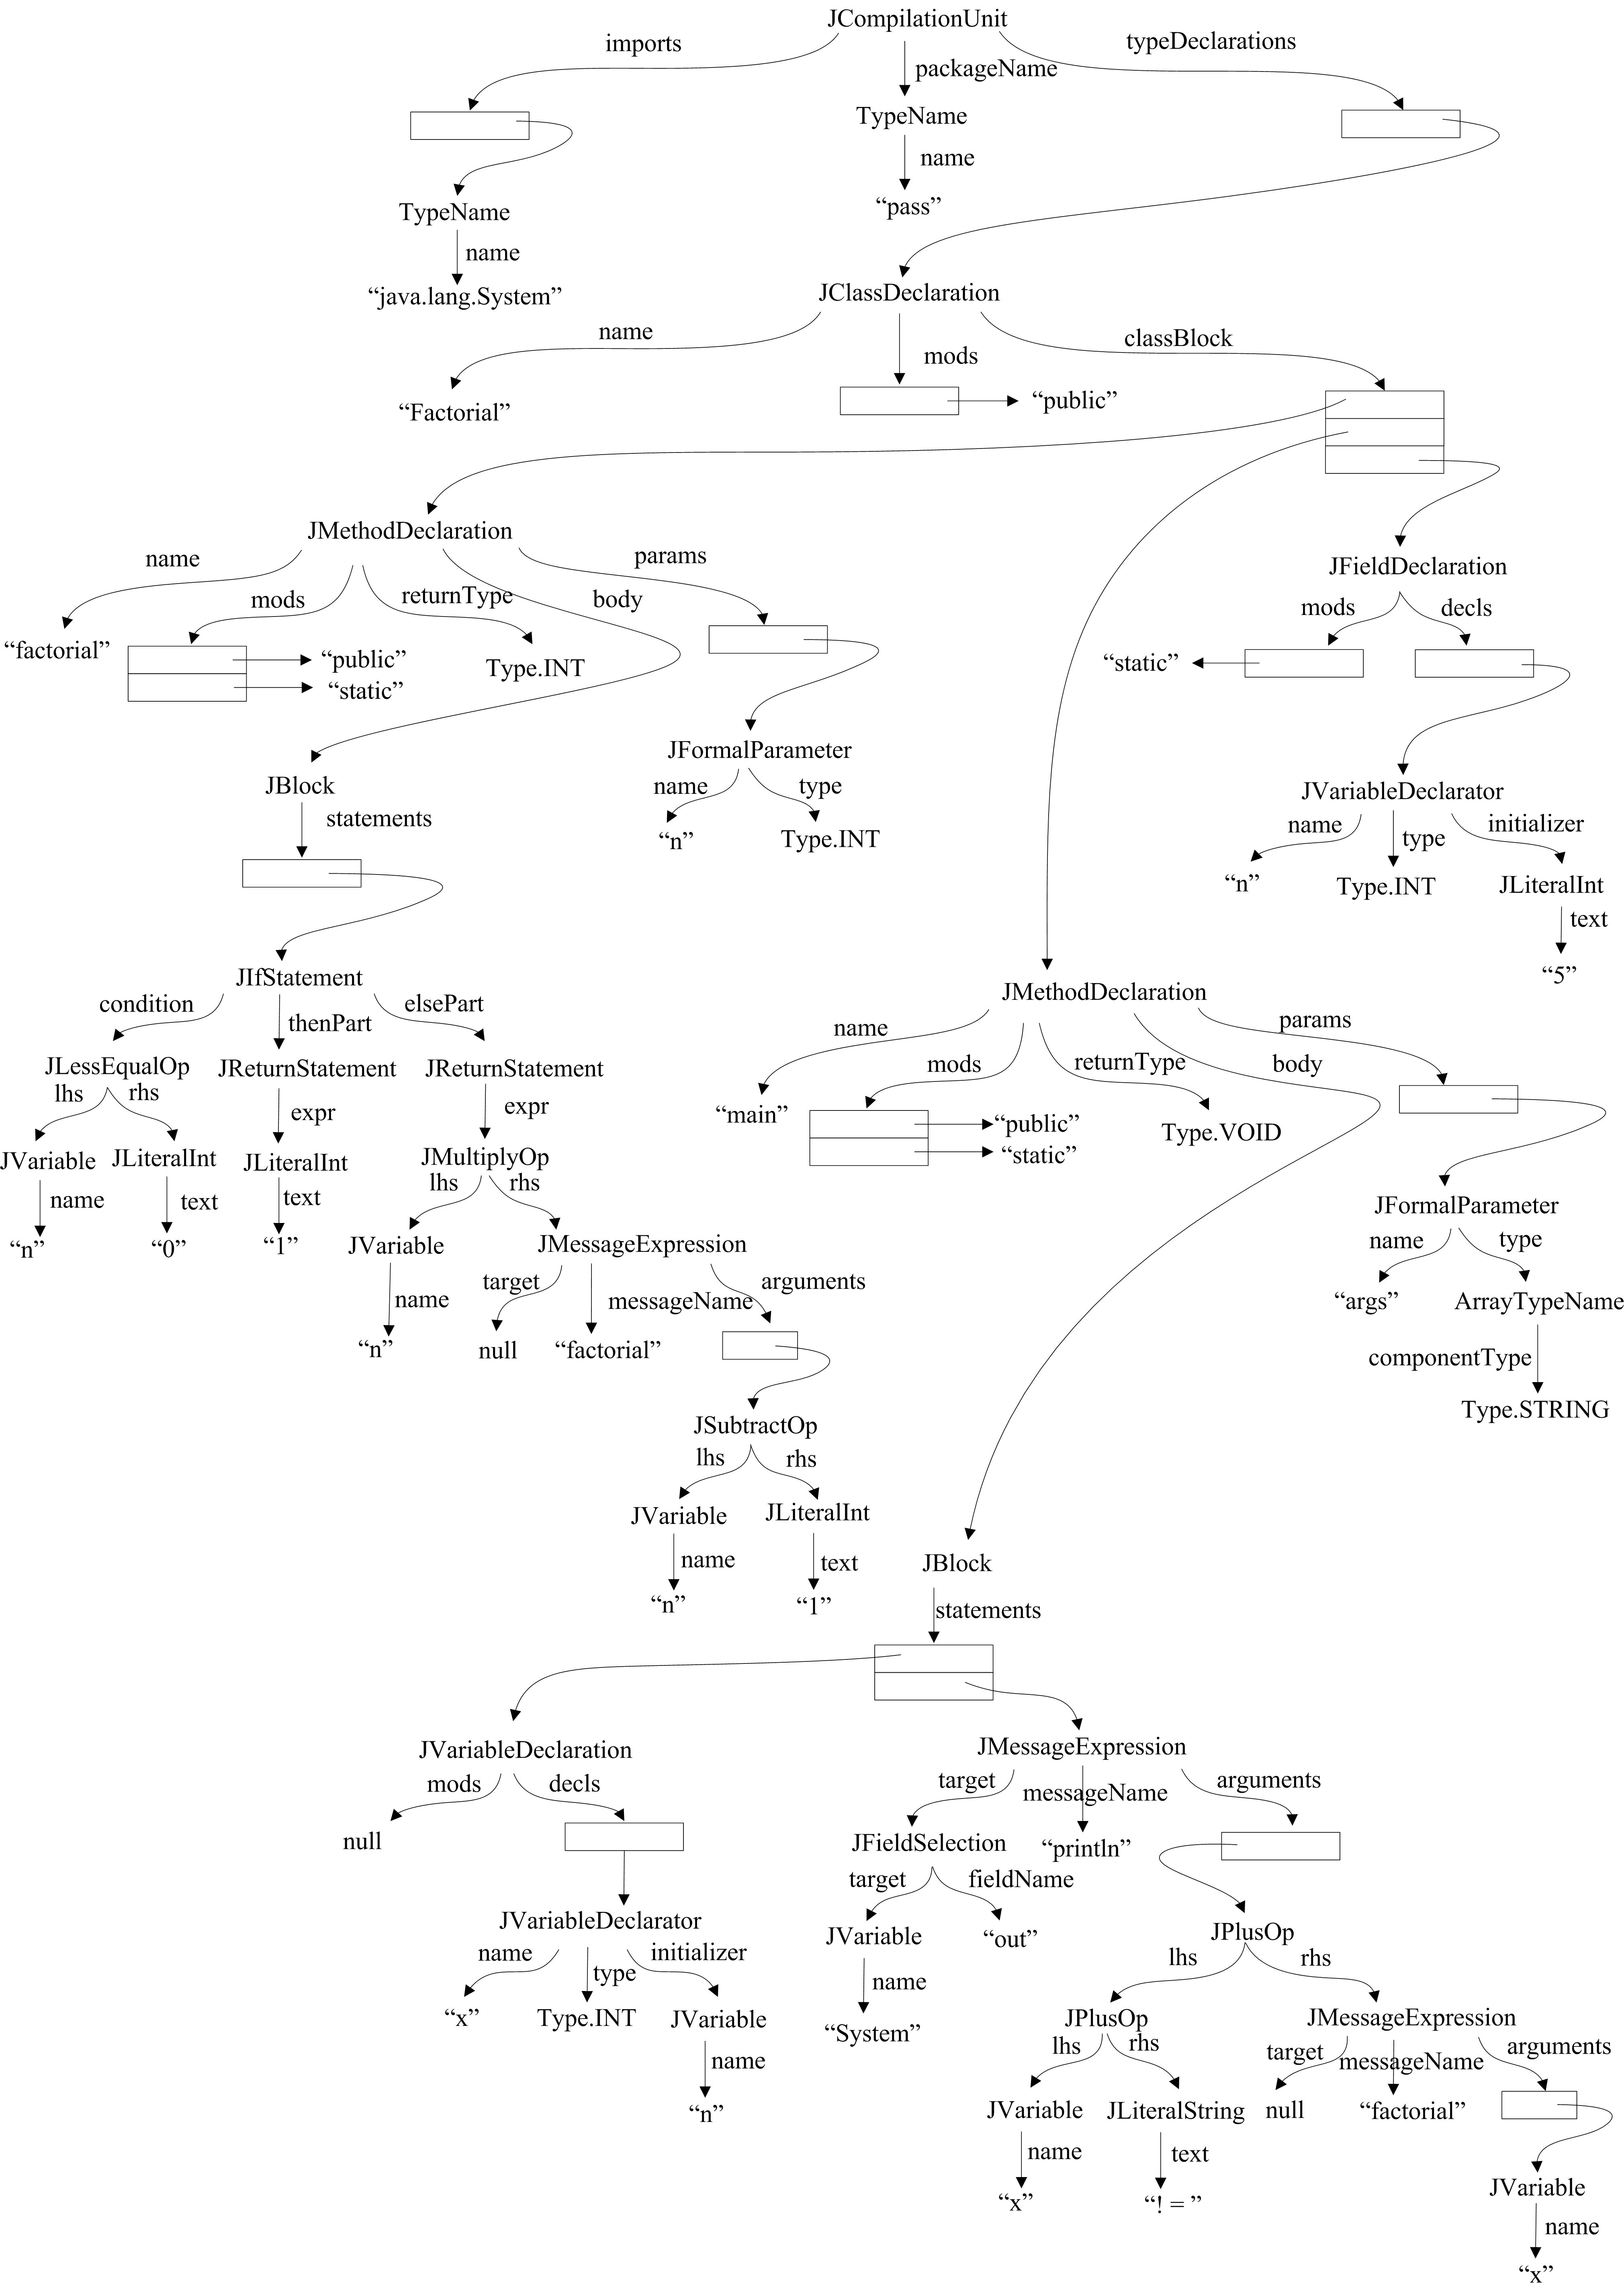
\includegraphics[scale=0.29]{{figures/figure03.01}.jpg}}
\end{center}
\end{frame}

\begin{frame}[fragile]
\pause

The nodes in the AST represent syntactic objects

\pause
\bigskip

The AST is rooted at a \lstinline{JCompilationUnit}, the syntactic object representing the program that we are compiling

\pause
\bigskip

The directed edges are labeled by the names of the fields they represent; for example, \lstinline{JCompilationUnit} has a package name, a list (an \lstinline{ArrayList}) of imported types, and a list (an \lstinline{ArrayList}) of class declarations

\pause
\bigskip

We are interested in a tree representation for our program because it is easier to analyze and decorate (with type information) a tree than it is to do the same with text

\pause
\bigskip

The AST makes the syntax implicit in the program text, explicit, which is essentially the purpose of parsing
\end{frame}

\section{Context-free Grammars and Languages}
\begin{frame}[fragile]
\pause

The grammars that we use to describe programming languages are inherently recursive and are best described by what we call context-free grammars, using a notation called Backus-Naur Form (BNF)

\pause
\bigskip

For example, the context-free rule

\text{ }
\begin{spaced}
\begin{production}
\mm{S} ::=  \lstinline{if} \lstinline{(}\mm{E}\lstinline{)} \mm{S}
\end{production}
\end{spaced}

\noindent says that, if \mm{E} is an expression and \mm{S} is a statement, then 

\text{ }
\begin{spaced}
\begin{production}
\lstinline{if} \lstinline{(}\mm{E}\lstinline{)} \mm{S}
\end{production}
\end{spaced}

\noindent is also a statement

\pause
\bigskip

There are abbreviations possible in the notation; for example, we can write

\text{ }
\begin{spaced}
\begin{production}
\mm{S} ::= \lstinline{if} \lstinline{(}\mm{E}\lstinline{)} \mm{S}
      \mm{|} \lstinline{if} \lstinline{(}\mm{E}\lstinline{)} \mm{S} \lstinline{else} \mm{S}
\end{production}
\end{spaced}

\noindent as shorthand for

\text{ }
\begin{spaced}
\begin{production}
\mm{S} ::= \lstinline{if} \lstinline{(}\mm{E}\lstinline{)} \mm{S}
\mm{S} ::= \lstinline{if} \lstinline{(}\mm{E}\lstinline{)} \mm{S} \lstinline{else} \mm{S}
\end{production}
\end{spaced}
\end{frame}

\begin{frame}[fragile]
\pause

Square brackets indicate that a phrase is optional; for example, the two rules from above can be written as

\text{ }
\begin{spaced}
\begin{production}
\mm{S} ::=  \lstinline{if} \lstinline{(}\mm{E}\lstinline{)} \mm{S} [\lstinline{else} \mm{S}]
\end{production}
\end{spaced}

\pause
\bigskip

Curly braces denote the Kleene closure, indicating that the phrase may appear zero or more times; for example

\text{ }
\begin{spaced}
\begin{production}
\mm{E} ::= \mm{T} \{\lstinline{\+} \mm{T}\}
\end{production}
\end{spaced}

\noindent says that an expression $E$ may be written as a term $T$, followed by zero or more  occurrences of \lstinline{+} followed by a term $T$, such as

\text{ }
\begin{spaced}
\begin{production}
\mm{T} \lstinline{+} \mm{T} \lstinline{+} \mm{T} \mm{\dots}
\end{production}
\end{spaced}

\pause

One may use the alternation sign $|$ inside right-hand-sides, using parentheses for grouping; for example

\text{ }
\begin{spaced}
\begin{production}
\mm{E} ::= \mm{T} \{(\lstinline{\+} \mm{|} \lstinline{\-}) \mm{T}\}
\end{production}
\end{spaced}

\noindent means that the additive operator may be either \lstinline{+} or \lstinline{-}, such as

\text{ }
\begin{spaced}
\begin{production}
\mm{T} \lstinline{+} \mm{T} \lstinline{\-} \mm{T} \lstinline{+} \mm{T}
\end{production}
\end{spaced}
\end{frame}

\begin{frame}[fragile]
\pause

BNF allows us to describe such syntax as that for a \jmm compilation unit

\text{ }
\begin{spaced}
\begin{production}
compilationUnit ::= [\lstinline{package} qualifiedIdentifier \lstinline{;}]
                           \{\lstinline{import}  qualifiedIdentifier \lstinline{;}\}
                           \{typeDeclaration\} \lstinline{EOF}
\end{production}
\end{spaced}

\pause
\bigskip

A context-free grammar\index{context-free grammar|textbf} is a tuple, $G = (N,T,S,P)$ where 
\begin{itemize}
\item $N$ is a set of non-terminal symbols, sometimes called non-terminals, 
\item $T$ is a set of terminal symbols, sometimes called terminals,
\item $S \in N$ is a designated non-terminal, called the start symbol, and
\item $P$ is a set of production rules, sometimes called productions or rules
\end{itemize}

\pause
\bigskip

For example, a context-free grammar that describes simple arithmetic expressions is $G = (N, T, S, P)$ where $N = \{E, T, F\}$ is the set of non-terminals, $T = \{\text{\lstinline{+}, \lstinline{*}, \lstinline{(}, \lstinline{)}, \lstinline{id}}\}$ is the set of terminals, $S = E$ is the start symbol, and

\text{ }
\begin{spaced}
\begin{production}
\mm{P} = \{\mm{E} ::= \mm{E} \lstinline{+} \mm{T},
        \mm{E} ::= \mm{T},
        \mm{T} ::= \mm{T} \lstinline{*} \mm{F},
        \mm{T} ::= \mm{F},
        \mm{F} ::= \lstinline{(}\mm{E}\lstinline{)},
        \mm{F} ::= \lstinline{id}\}
\end{production}
\end{spaced}
\end{frame}

\begin{frame}[fragile]
\pause

We can denote the above grammar a little less formally, simply as a sequence of production rules

\text{ }
\begin{spaced}
\begin{production}
\mm{E} ::= \mm{E} \lstinline{+} \mm{T}
\mm{E} ::= \mm{T}
\mm{T} ::= \mm{T}  \lstinline{*} {F}
\mm{T} ::= \mm{F}
\mm{F} ::= \lstinline{(}\mm{E}\lstinline{)}
\mm{F} ::= \lstinline{id}
\end{production}
\end{spaced}

\pause
\bigskip

The start symbol is important because it is from this symbol, using the production rules, that we can generate strings in a language

\pause
\bigskip

For example, we can record a sequence of applications of the production rules, starting from $E$ (starting symbol in the above grammar) to the sentence \lstinline{id + id * id} as follows

\text{ }
\begin{spaced}
\begin{production}
\mm{E} \mm{\Rightarrow} \mm{E} \lstinline{+} \mm{T}
   \mm{\Rightarrow} \mm{T} \lstinline{+} \mm{T}
   \mm{\Rightarrow} \mm{F} \lstinline{+} \mm{T}
   \mm{\Rightarrow} id \lstinline{+} \mm{T}
   \mm{\Rightarrow} id \lstinline{+} \mm{T} \lstinline{*} \mm{F}
   \mm{\Rightarrow} id \lstinline{+} \mm{F} \lstinline{*} \mm{F}
   \mm{\Rightarrow} \lstinline{id + id *} \mm{F}
   \mm{\Rightarrow} \lstinline{id + id * id}
\end{production}
\end{spaced}
\end{frame}

\begin{frame}[fragile]
\pause

When one string can be re-written as another string, using zero or more production rules from the grammar, we say the first string derives ($\derives$) the second string

\pause
\bigskip
 
For example

\text{ }
\begin{spaced}
\begin{production}
\mm{E} \mm{\derives} \mm{E} (in zero steps)
\mm{E} \mm{\derives} \lstinline{id} \lstinline{+} \mm{F} \lstinline{*} \mm{F}
\mm{T} \lstinline{+} \mm{T} \mm{\derives}  \lstinline{id + id * id}
\end{production}
\end{spaced}

\pause
\bigskip

We say the language $L(G)$ that is described by a grammar $G$ consists of all the strings (sentences) comprised of only terminal symbols, that can be derived from the start symbol, ie, $L(G) = \{w | S \derives w \text{ and } w \in T*\}$

\pause
\bigskip

For example, in the grammar above

\text{ }
\begin{spaced}
\begin{production}
\mm{E \derives} \lstinline{id + id * id}
\mm{E \derives} \lstinline{id}
\mm{E \derives} \lstinline{(id + id)} \lstinline{* id}
\end{production}
\end{spaced}

\noindent so,  $L(G)$ includes each of

\text{ }
\begin{spaced}
\begin{production}
\lstinline{id + id * id}
\lstinline{id}
\lstinline{(id + id)} \lstinline{* id}
\end{production}
\end{spaced}

\noindent and infinitely more finite sentences
\end{frame}

\begin{frame}[fragile]
\pause

We are interested in languages consisting of strings of terminals that can be derived from a grammar's start symbol

\pause
\bigskip

There are two kinds of derivation that will be important to us when we go about parsing these languages: left-most derivations and right-most derivations

\pause
\bigskip

A left-most derivation is a derivation in which at each step, the next string is derived by applying a production rule for rewriting the left-most non-terminal

\pause
\bigskip

For example

\text{ }
\begin{spaced}
\begin{production}
\underline{\mm{E}} \mm{\Rightarrow} \underline{\mm{E}} \lstinline{+} \mm{T}
   \mm{\Rightarrow} \underline{\mm{T}} \lstinline{+} \mm{T}
   \mm{\Rightarrow} \underline{\mm{F}} \lstinline{+} \mm{T}
   \mm{\Rightarrow} id \lstinline{+} \underline{\mm{T}}
   \mm{\Rightarrow} id \lstinline{+} \underline{\mm{T}} \lstinline{*} \mm{F}
   \mm{\Rightarrow} id \lstinline{+} \underline{\mm{F}} \lstinline{*} \mm{F}
   \mm{\Rightarrow} \lstinline{id + id *} \underline{\mm{F}}
   \mm{\Rightarrow} \lstinline{id + id * id}
\end{production}
\end{spaced}
\end{frame}

\begin{frame}[fragile]
\pause

A right-most derivation is a derivation in which at each step, the next string is derived by applying a production rule for rewriting the right-most non-terminal

\pause
\bigskip

For example, the right-most derivation of \lstinline{id + id * id} would go as follows

\text{ }
\begin{spaced}
\begin{production}
\underline{\mm{E}} \mm{\Rightarrow} \mm{E} \lstinline{+} \underline{\mm{T}}
   \mm{\Rightarrow} \mm{E} \lstinline{+} \mm{T} \lstinline{*} \underline{\mm{F}}
   \mm{\Rightarrow} \mm{E} \lstinline{+} \underline{\mm{T}} \lstinline{*} \lstinline{id}
   \mm{\Rightarrow} \mm{E} \lstinline{+} \underline{\mm{F}} \lstinline{*} \lstinline{id}
   \mm{\Rightarrow} \underline{\mm{E}} \lstinline{+ id * id}
   \mm{\Rightarrow} \underline{\mm{T}} \lstinline{+ id * id}
   \mm{\Rightarrow} \underline{\mm{F}} \lstinline{+ id * id}
   \mm{\Rightarrow} \lstinline{id + id * id}
\end{production}
\end{spaced}

\pause

We use the term sentential form to refer to any string of (terminal and non-terminal) symbols that can be derived from the start symbol

\pause
\bigskip

For example, in the previous derivation

\text{ }
\begin{spaced}
\begin{production}
\mm{E}
\mm{E} \lstinline{+} \mm{T}
\mm{E} \lstinline{+} \mm{T} \lstinline{*} \mm{F}
\mm{E} \lstinline{+} \mm{T} \lstinline{* id}
\mm{E} \lstinline{+} \mm{F} \lstinline{* id}
\mm{E} \lstinline{+ id * id}
\mm{T} \lstinline{+ id * id}
\mm{F} \lstinline{+ id * id}
\lstinline{id + id * id}
\end{production}
\end{spaced}
\end{frame}

\begin{frame}[fragile]
\pause

An alternative representation of a derivation is the parse tree, a tree that illustrates the derivation and the structure of an input string (at the leaves) from a start symbol (at the root)

\pause
\bigskip

For example, the following figure shows the parse tree for \lstinline{id + id * id}.

\begin{center}
\visible<3->{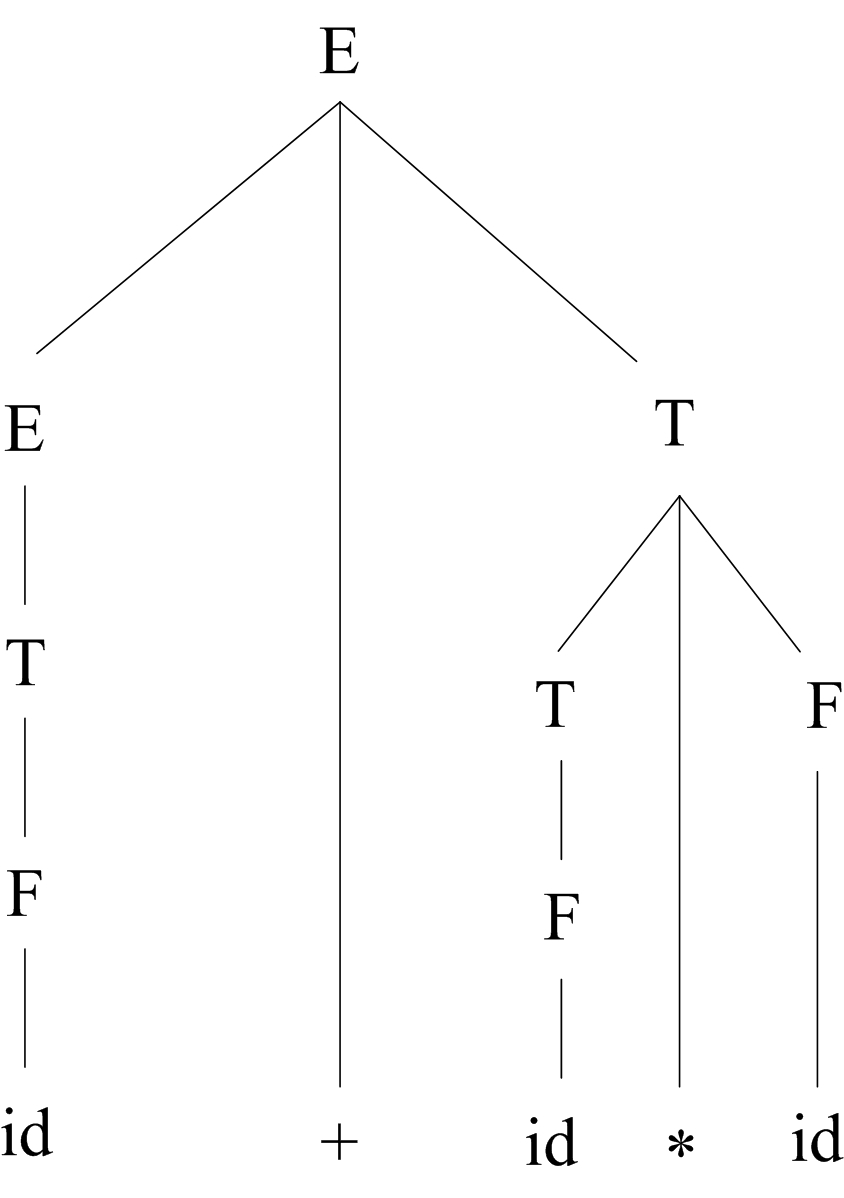
\includegraphics[scale=0.6]{{figures/figure03.02}.jpg}}
\end{center}

\pause
\bigskip

Given a grammar $G$, if there exists a sentence $s$ in $L(G)$ for which there are more than one left-most derivations in $G$ (or equivalently, either more than one right-most derivations, or more than one parse tree for $s$ in $G$), we say that the sentence $s$ is ambiguous

\pause
\bigskip

If a grammar $G$ describes at least one ambiguous sentence, the grammar $G$ is an ambiguous grammar; if there is no such sentence, we say the grammar is unambiguous
\end{frame}

\begin{frame}[fragile]
\pause

Consider the grammar

\text{ }
\begin{spaced}
\begin{production}
\mm{E} ::= \mm{E} \lstinline{+} \mm{E} \mm{|} \mm{E} \lstinline{*} \mm{E} \mm{|} \lstinline{(}\mm{E}\lstinline{)} \mm{|} \lstinline{id}
\end{production}
\end{spaced}

\noindent and, consider the sentence \lstinline{id + id * id}

\pause
\bigskip

One left-most derivation for this sentence is

\text{ }
\begin{spaced}
\begin{production}
\underline{\mm{E}} \mm{\Rightarrow} \underline{\mm{E}} \lstinline{+} \mm{E}
   \mm{\Rightarrow} \lstinline{id +} \underline{\mm{E}}
   \mm{\Rightarrow} \lstinline{id +} \underline{\mm{E}} \lstinline{*} \mm{E}
   \mm{\Rightarrow} \lstinline{id + id *} \underline{\mm{E}}
   \mm{\Rightarrow} \lstinline{id + id * id}
\end{production}
\end{spaced}

\pause
\bigskip

Another left-most derivation of the same sentence is

\text{ }
\begin{spaced}
\begin{production}
\underline{\mm{E}} \mm{\Rightarrow} \underline{\mm{E}} \lstinline{*} \mm{E}
   \mm{\Rightarrow} \underline{\mm{E}} \lstinline{+} \mm{E} \lstinline{*} \mm{E}
   \mm{\Rightarrow} \lstinline{id +} \underline{\mm{E}} \lstinline{*} \mm{E}
   \mm{\Rightarrow} \lstinline{id + id *} \underline{\mm{E}}
   \mm{\Rightarrow} \lstinline{id + id * id}
\end{production}
\end{spaced}

\pause
\bigskip

Therefore, the grammar is ambiguous
\end{frame}

\begin{frame}[fragile]
\pause

The above sentence also has two right-most derivations in the grammar

\text{ }
\begin{spaced}
\begin{production}
\underline{\mm{E}} \mm{\Rightarrow} \mm{E} \lstinline{+} \underline{\mm{E}}
   \mm{\Rightarrow} \mm{E} \lstinline{+} \mm{E} \lstinline{*} \underline{\mm{E}}
   \mm{\Rightarrow} \mm{E} \lstinline{+} \underline{\mm{E}} \lstinline{* id}
   \mm{\Rightarrow} \underline{\mm{E}} \lstinline{+ id * id}
   \mm{\Rightarrow} \lstinline{id + id * id}
\end{production}
\end{spaced}

\noindent and

\text{ }
\begin{spaced}
\begin{production}
\underline{\mm{E}} \mm{\Rightarrow} \mm{E} \lstinline{*} \underline{\mm{E}}
   \mm{\Rightarrow} \underline{\mm{E}} \lstinline{* id}
   \mm{\Rightarrow} \mm{E} \lstinline{+} \underline{\mm{E}} \lstinline{* id}
   \mm{\Rightarrow} \underline{\mm{E}} \lstinline{+ id * id}
   \mm{\Rightarrow} \lstinline{id + id * id}
\end{production}
\end{spaced}

\noindent with the following two parse trees
\begin{center}
\visible<2->{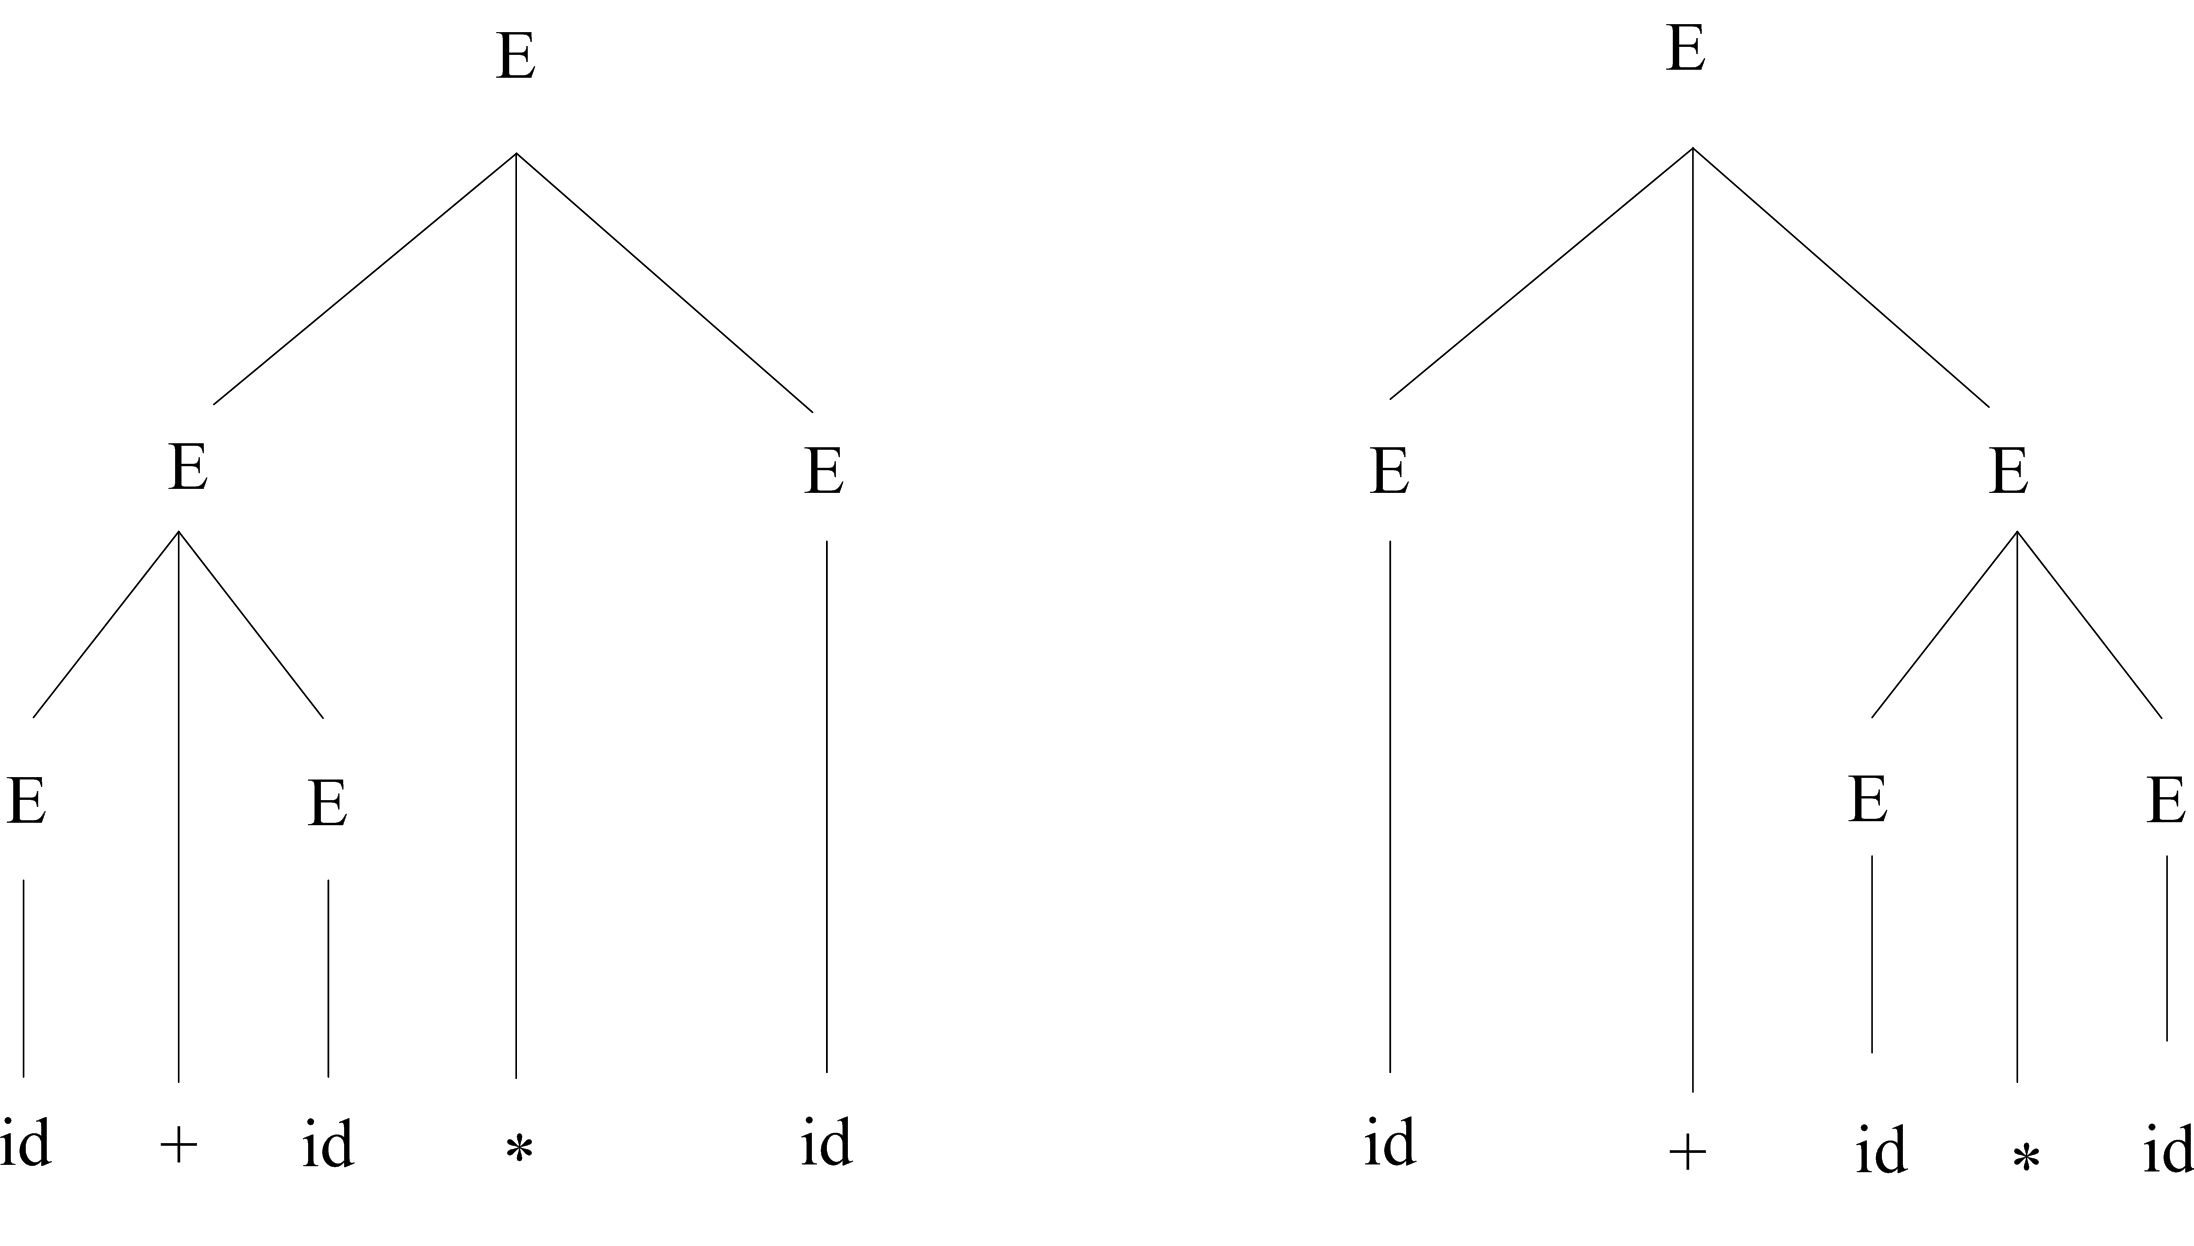
\includegraphics[scale=0.4]{{figures/figure03.03}.jpg}}
\end{center}
\end{frame}

\begin{frame}[fragile]
\pause

As another example, consider the grammar describing conditional statements

\text{ }
\begin{spaced}
\begin{production}
\mm{S} ::= \lstinline{if} \lstinline{(}\mm{E}\lstinline{)} \mm{S}
      \mm{|} \lstinline{if} \lstinline{(}\mm{E}\lstinline{)} \mm{S} \lstinline{else} \mm{S}
      \mm{|} \lstinline{s}
\mm{E} ::=  \lstinline{e}
\end{production}
\end{spaced}

and consider the sentence

\text{ }
\begin{spaced}
\begin{production}
\lstinline{if (e)} \lstinline{if (e)} \lstinline{s else s}
\end{production}
\end{spaced}
\end{frame}

\begin{frame}[fragile]
\pause

There exist two left-most derivations for the above sentence in the grammar

\text{ }
\begin{spaced}
\begin{production}
\underline{\mm{S}} \mm{\Rightarrow} \lstinline{if} \lstinline{(}\underline{\mm{E}}\lstinline{)} \mm{S} \lstinline{else} \mm{S}
   \mm{\Rightarrow} \lstinline{if} \lstinline{(e)} \underline{\mm{S}} \lstinline{else} \mm{S}
   \mm{\Rightarrow} \lstinline{if} (e) \lstinline{if} \lstinline{(}\underline{\mm{E}}\lstinline{)} \mm{S} \lstinline{else} \mm{S}
   \mm{\Rightarrow} \lstinline{if} (e) \lstinline{if} \lstinline{(e)} \underline{\mm{S}} \lstinline{else} \mm{S}
   \mm{\Rightarrow} \lstinline{if} \lstinline{(e)} \lstinline{if} \lstinline{(e) s} \lstinline{else} \underline{\mm{S}}
   \mm{\Rightarrow} \lstinline{if} \lstinline{(e)} \lstinline{if} \lstinline{(e) s} \lstinline{else} \lstinline{s}
\end{production}
\end{spaced}

\noindent and

\text{ }
\begin{spaced}
\begin{production}
\underline{\mm{S}} \mm{\Rightarrow} \lstinline{if} \lstinline{(}\underline{\mm{E}}\lstinline{)} \mm{S}
   \mm{\Rightarrow} \lstinline{if} \lstinline{(e)} \underline{\mm{S}}
   \mm{\Rightarrow} \lstinline{if} \lstinline{(e)} \lstinline{if} \lstinline{(}\underline{\mm{E}}\lstinline{)} \mm{S} \lstinline{else} \mm{S}
   \mm{\Rightarrow} \lstinline{if} \lstinline{(e)} \lstinline{if} \lstinline{(e)} \underline{\mm{S}} \lstinline{else} \mm{S}
   \mm{\Rightarrow} \lstinline{if} \lstinline{(e)} \lstinline{if} \lstinline{(e)} \lstinline{s} \lstinline{else} \underline{\mm{S}}
   \mm{\Rightarrow} \lstinline{if} \lstinline{(e)} \lstinline{if} \lstinline{(e) s} \lstinline{else} \lstinline{s}
\end{production}
\end{spaced}

\noindent with the following parse trees

\begin{center}
\visible<2->{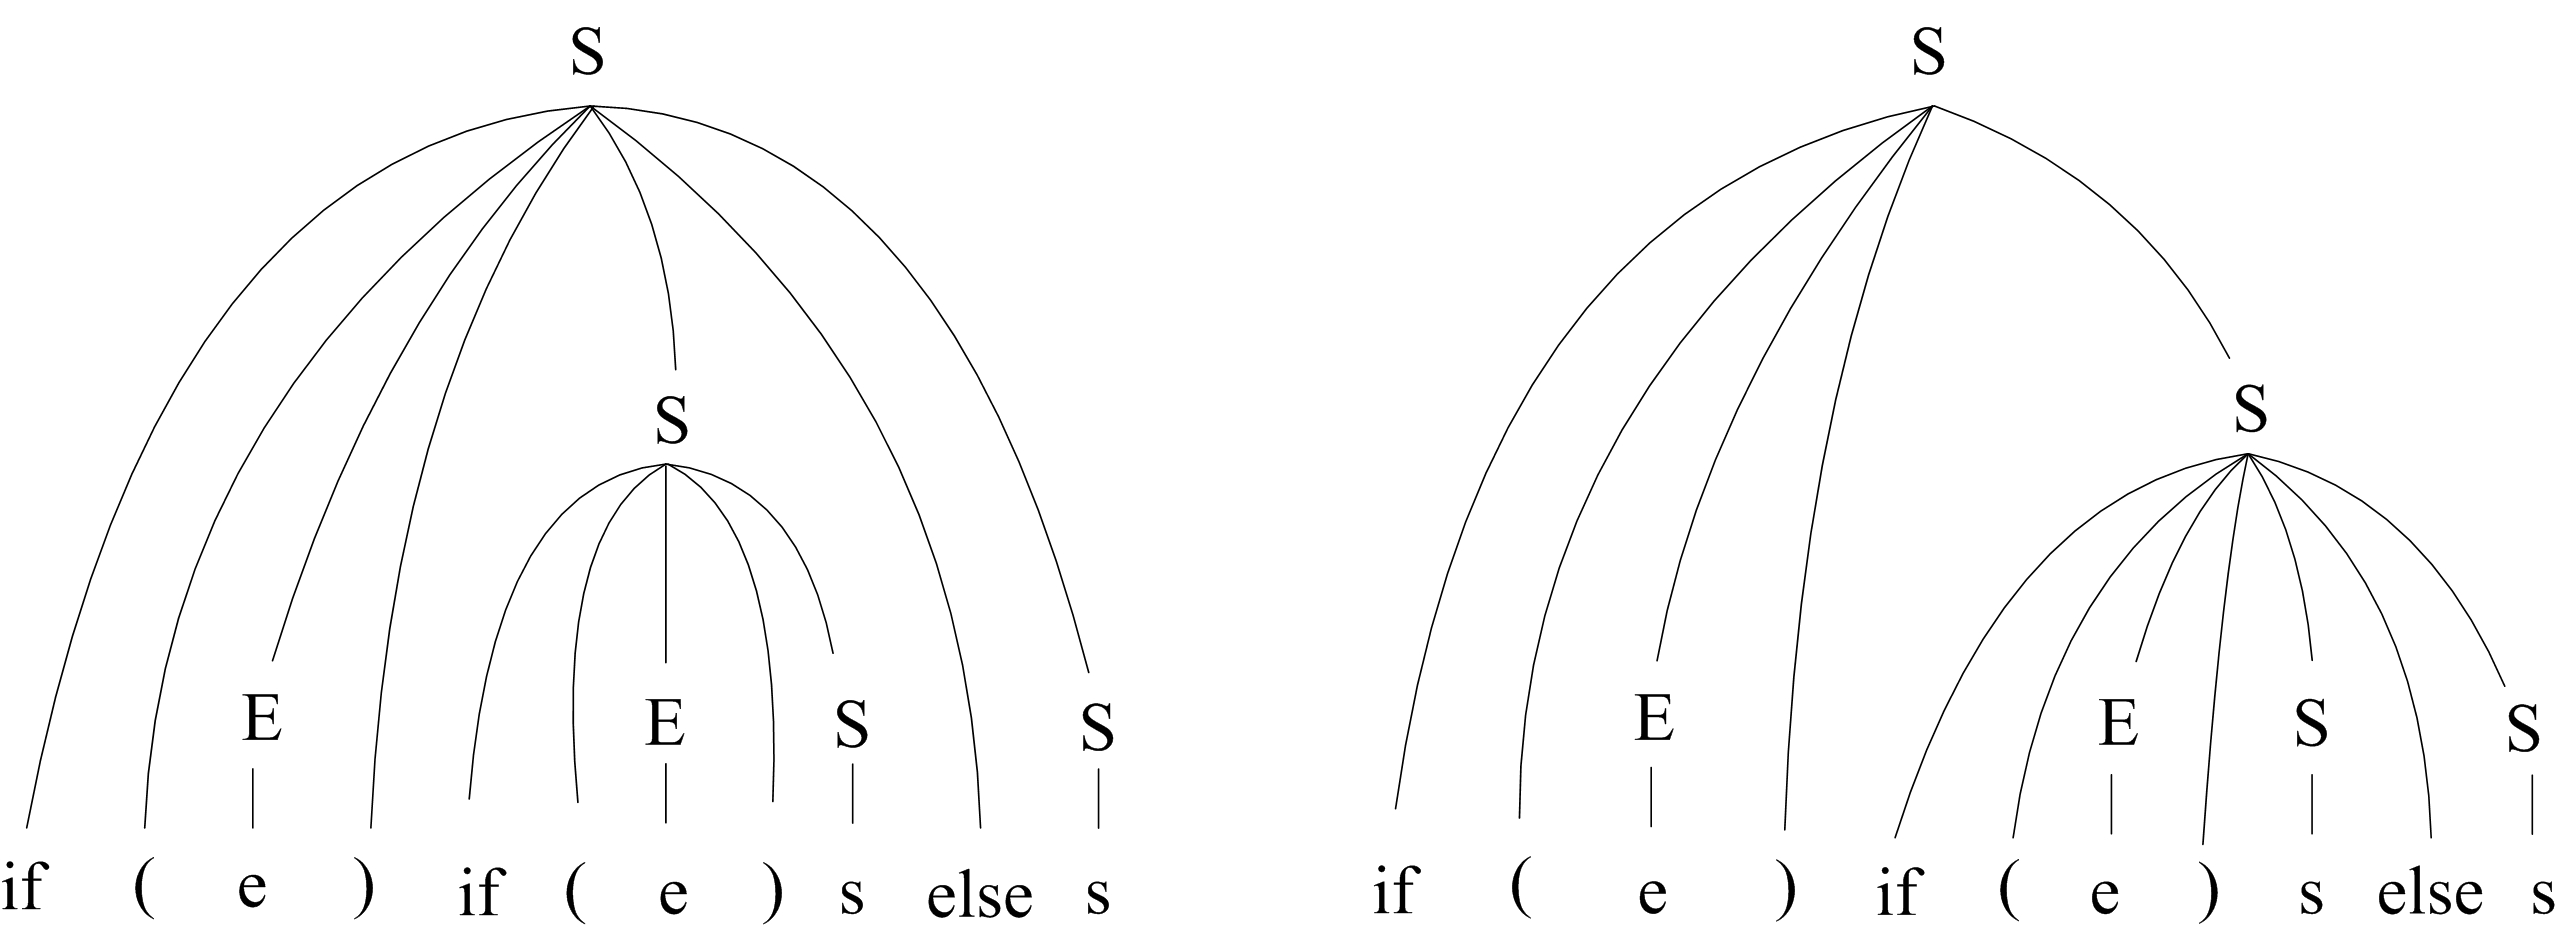
\includegraphics[scale=0.4]{{figures/figure03.04}.jpg}}
\end{center}
\end{frame}

\begin{frame}[fragile]
\pause

One could easily modify the syntax of conditionals to remove the ambiguity

\text{ }
\begin{spaced}
\begin{production}
\mm{S} ::= \lstinline{if} \mm{E} \lstinline{do} \mm{S}
      \mm{|} \lstinline{if} \mm{E} \lstinline{then} \mm{S} \lstinline{else} \mm{S}
      \mm{|} \lstinline{s}
\mm{E} ::= \lstinline{e}
\end{production}
\end{spaced}

\pause
\bigskip

But programmers have become both accustomed to (and fond of) the ambiguous conditional

\pause
\bigskip

Compiler writers handle the rule as a special case in the compiler's parser, making sure that an \lstinline{else} is grouped along with the closest preceding \lstinline{if}
\end{frame}

\begin{frame}[fragile]
\pause

The \jmm grammar (and the Java grammar) have another ambiguity, which is even more difficult; consider the problem of parsing the expression \lstinline{x.y.z.w}

\pause
\bigskip

Clearly \lstinline{w} is a field; if it were a method expression, then that would be evident in the syntax \lstinline{x.y.z.w()}

\pause
\bigskip

But, what about \lstinline{x.y.z}?  There are several possibilities depending on the types of the names \lstinline{x}, \lstinline{y} and \lstinline{z}

\begin{itemize}
\item If \lstinline{x} is the name of a local variable, it might refer to an object with a field \lstinline{y}, referring to another object with a field \lstinline{z}, referring to yet another object having our field \lstinline{w}; in this case, the expression would be parsed as a cascade of field selection expressions

\item Alternatively, \lstinline{x.y} might be the name of a package, in which the class \lstinline{z} is defined; in this case, we would parse the expression by first parsing \lstinline{x.y.z} as a fully qualified class and then parse \lstinline{w} as a static field selection of that class

\item Other possibilities, parsing various permutations of (possibly qualified) class names and field selection operations, also exist
\end{itemize}

\pause
\bigskip

The parser cannot determine how the expression \lstinline{x.y.z} is parsed because types are not decided until after it has parsed the program and constructed its AST, so represents \lstinline{x.y.z} in the AST by an \lstinline{AmbiguousName} node; later on, after type declarations have been processed, the compiler re-writes this node as the appropriate sub-tree
\end{frame}

\section{Top-down Deterministic Parsing}
\begin{frame}[fragile]
\pause

There are two popular top-down deterministic parsing strategies: parsing by recursive descent and LL(1) parsing; both scan the input from left to right, looking at and scanning just one symbol at a time

\pause
\bigskip

The parser starts with the grammar's start symbol as an initial goal in the parsing process, which is then rewritten using a BNF rule replacing the symbol with the right-hand-side sequence of symbols

\pause
\bigskip

For example, in parsing a \jmm program, our initial goal is to parse the start symbol, compilationUnit, which is defined by the following BNF rule

\text{ }
\begin{spaced}
\begin{production}
compilationUnit ::= [\lstinline{package} qualifiedIdentifier \lstinline{;}]
                           \{\lstinline{import}  qualifiedIdentifier \lstinline{;}\}
                           \{typeDeclaration\} \lstinline{EOF}
\end{production}
\end{spaced}

\pause
\bigskip

The goal of parsing a compilationUnit in the input can be rewritten as a number of sub-goals

\begin{enumerate}
\item If there is a \lstinline{package} statement in the input sentence, then we parse that
\item If there are \lstinline{import} statements in the input, then we parse them
\item If there are any type declarations, then we parse them
\item Finally, we parse the terminating \lstinline{EOF} token
\end{enumerate}
\end{frame}

\begin{frame}[fragile]
\pause

Parsing a token, like \lstinline{package}, is simple enough; if we see it, we simply scan it

\pause
\bigskip

Parsing a non-terminal is treated as another parsing (sub-) goal

\pause
\bigskip

For example, in the \lstinline{package} statement, once we have scanned the \lstinline{package} token, we are left with parsing a qualifiedIdentifier, which is defined by the following BNF rule

\text{ }
\begin{spaced}
\begin{production}
qualifiedIdentifier ::= \lstinline{\<identifier\>} \{\lstinline{\.} \lstinline{\<identifier\>}\}
\end{production}
\end{spaced}

\pause

We scan an \lstinline{<identifier>} (treated by the lexical scanner as a token), and, so long as we see another period in the input, we scan that period and scan another \lstinline{<identifier>}

\pause
\bigskip

That we start at the start symbol, and continually rewrite non-terminals using BNF rules until we eventually reach leaves (the tokens are the leaves) makes this a top-down parsing technique

\pause
\bigskip

Since at each step in parsing a non-terminal, we replace a parsing goal with a sequence of sub-goals, we often call this a goal-oriented parsing technique
\end{frame}

\begin{frame}[fragile]
\pause

How do we decide what next step to take? For example, how do we decide whether or not there are more \lstinline{import} statements to parse? 

\pause
\bigskip

We decide by looking at the next un-scanned input token; if it is an \lstinline{import}, we have another \lstinline{import} statement to parse; otherwise we go on to parsing type declarations

\pause
\bigskip

As another example, consider the definition for the statement non-terminal

\text{ }
\begin{spaced}
\begin{production}
statement ::= block
                  \mm{|} \lstinline{if} parExpression statement [\lstinline{else} statement]
                  \mm{|} \lstinline{while} parExpression statement
                  \mm{|} \lstinline{return} [expression] \lstinline{;}
                  \mm{|} \lstinline{;}
                  \mm{|} statementExpression \lstinline{;}
\end{production}
\end{spaced}

\pause
\bigskip

We have six alternatives to choose from, depending on the next un-scanned input token

\begin{enumerate}
\item if the next token is a \lstinline${$, we parse a block
\item if the next token is an \lstinline{if}, we parse an \lstinline{if} statement
\item if the next token is a \lstinline{while}, we parse a \lstinline{while} statement
\item if the next token is a \lstinline{return}, we parse a \lstinline{return} statement
\item if the next token is a semicolon, we parse an empty statement
\item otherwise, we parse a statementExpression
\end{enumerate}
\end{frame}

\begin{frame}[fragile]
\pause

In the above example, the decision could be made by looking at the next single un-scanned input token; when this is the case, we say that our grammar is LL(1)

\pause
\bigskip

In some cases, one must lookahead several tokens in the input to decide which alternative to take

\pause
\bigskip

In all cases, because we can predict which of several alternative right-hand-sides of a BNF rule to apply, based on the next input token(s), we say this is a predictive parsing technique

\pause
\bigskip

There are two principal top-down (goal-oriented, or predictive) parsing techniques available to us
\begin{enumerate}
\item Parsing by recursive descent
\item LL(1) or LL($k$) parsing
\end{enumerate}
\end{frame}

\begin{frame}[fragile]
\pause

Parsing by recursive descent involves writing a method (or procedure) for parsing each non-terminal according to the production rules that define that non-terminal

\pause
\bigskip

Depending on the next un-scanned input symbol, the method decides which rule to apply and then scans any terminals (tokens) on the right hand side by calling upon the \lstinline{Scanner}, and parses any non-terminals by recursively invoking the methods that parse them

\pause
\bigskip

This is the strategy we use in parsing \jmm programs

\pause
\bigskip

We already saw the method \lstinline{compilationUnit()} that parses a \jmm \lstinline{compilationUnit}

\pause
\bigskip

As another example, consider the rule defining qualifiedIdentifier

\text{ }
\begin{spaced}
\begin{production}
qualifiedIdentifier ::= \lstinline{\<identifier\>} \{\lstinline{\.} \lstinline{\<identifier\>}\}
\end{production}
\end{spaced}

\pause

Parsing a qualifiedIdentifier such as \lstinline{java.lang.Class} is straightforward
\begin{enumerate}
\item We look at the next incoming token and if it is an identifier, we scan it; if it is not an identifier, then we raise an error
\item Repeatedly, so long as the next incoming token is a period
\begin{enumerate}[a.]
\item We scan the period
\item We look at the next incoming token and if it is an identifier, we scan it; otherwise, we raise an error
\end{enumerate}
\end{enumerate}
\end{frame}

\begin{frame}[fragile]
\pause

The method for parsing qualifiedIdentifier not only parses the input, but also constructs an AST node for recording the fully qualified name as a string

\begin{lstlisting}[language=Java]
    private TypeName qualifiedIdentifier() {
        int line = scanner.token().line();
        mustBe(IDENTIFIER);
        String qualifiedIdentifier = scanner.previousToken().image();
        while (have(DOT)) {
            mustBe(IDENTIFIER);
            qualifiedIdentifier += "." + scanner.previousToken().image();
        }
        return new TypeName(line, qualifiedIdentifier);
    }
\end{lstlisting}

\pause
\bigskip

The helper predicate method \lstinline{have()} looks at the next incoming token (supplied by the \lstinline{Scanner}), and if that token matches its argument, then it scans the token in the input and returns \lstinline{true}; otherwise, it scans nothing and returns \lstinline{false}

\pause
\bigskip

The helper method \lstinline{mustBe()} requires that the next incoming token match its argument; it looks at the next token and if it matches its argument, it scans that token in the input, and it raises an error otherwise

\pause
\bigskip

\lstinline{mustBe()} provides certain amount of error recovery as well
\end{frame}

\begin{frame}[fragile]
\pause

As another example, consider our syntax for statements

\text{ }
\begin{spaced}
\begin{production}
statement ::= block
                  \mm{|} \lstinline{if} parExpression statement [\lstinline{else} statement]
                  \mm{|} \lstinline{while} parExpression statement
                  \mm{|} \lstinline{return} [expression] \lstinline{;}
                  \mm{|} \lstinline{;}
                  \mm{|} statementExpression \lstinline{;}
\end{production}
\end{spaced}

\pause
\bigskip

The method for parsing a statement decides which rule to apply when looking at the next un-scanned token

\begin{lstlisting}[language=Java]
    private JStatement statement() {
        int line = scanner.token().line();
        if (see(LCURLY)) {
            return block();
        } else if (have(IF)) {
            JExpression test = parExpression();
            JStatement consequent = statement();
            JStatement alternate = have(ELSE) ? statement() : null;
            return new JIfStatement(line, test, consequent, alternate);
\end{lstlisting}
\end{frame}

\begin{frame}[fragile]
\pause

\begin{lstlisting}[language=Java]
        } else if (have(WHILE)) {
            JExpression test = parExpression();
            JStatement statement = statement();
            return new JWhileStatement(line, test, statement);
        } else if (have(RETURN)) {
            if (have(SEMI)) {
                return new JReturnStatement(line, null);
            } else {
                JExpression expr = expression();
                mustBe(SEMI);
                return new JReturnStatement(line, expr);
            }
        } else if (have(SEMI)) {
            return new JEmptyStatement(line);
        } else { // Must be a statementExpression
            JStatement statement = statementExpression();
            mustBe(SEMI);
            return statement;
        }
    }
\end{lstlisting}

\pause
\bigskip

The helper predicate method \lstinline{see()} simply looks at the incoming token and returns \lstinline{true} if it is the token that we are looking for, and \lstinline{false} otherwise; in no case is anything scanned
\end{frame}

\begin{frame}[fragile]
\pause

The parsing of statements works because we can determine which rule to follow in parsing the statement based only on the next un-scanned symbol in the input source

\pause
\bigskip

Unfortunately, this is not always the case

\pause
\bigskip

Sometimes we must consider the next few symbols in deciding what to do, ie, we must look ahead in the input stream of tokens to decide which rule to apply

\pause
\bigskip

For example, consider the syntax for a simple unary expression

\text{ }
\begin{spaced}
\begin{production}
simpleUnaryExpression ::= \lstinline{!} unaryExpression
                                   \mm{|} \lstinline{(} basicType \lstinline{)}  unaryExpression //cast
                                   \mm{|} \lstinline{(} referenceType \lstinline{)} simpleUnaryExpression // cast
                                   \mm{|} postfixExpression
\end{production}
\end{spaced}

\pause
\bigskip

For this, we must not only differentiate between the two kinds (basic type and reference type) of casts, but we must also distinguish a cast from a postfix expression that is a parenthesized expression; for example \lstinline{(x)}
\end{frame}

\begin{frame}[fragile]
\pause

Consider the code for parsing a simple unary expression

\begin{lstlisting}[language=Java]
    private JExpression simpleUnaryExpression() {
        int line = scanner.token().line();
        if (have(LNOT)) {
            return new JLogicalNotOp(line, unaryExpression());
        } else if (seeCast()) {
            mustBe(LPAREN);
            boolean isBasicType = seeBasicType();
            Type type = type();
            mustBe(RPAREN);
            JExpression expr = isBasicType
                ? unaryExpression()
                : simpleUnaryExpression();
            return new JCastOp(line, type, expr);
        } else {
            return postfixExpression();
        }
    }
\end{lstlisting}

\pause
\bigskip

We use the predicate \lstinline{seeCast()} to distinguish casts from parenthesized expressions, and \lstinline{seeBasicType()} to distinguish between casts to basic types from casts to reference types

\pause
\bigskip

Now, consider the two predicates

\begin{lstlisting}[language=Java]
    private boolean seeBasicType() {
        if (see(BOOLEAN) || see(CHAR) || see(INT)) {
            return true;
        } else {
            return false;
        }
    }
\end{lstlisting}
\end{frame}

\begin{frame}[fragile]
\pause

\begin{lstlisting}[language=Java]
    private boolean seeCast() {
	scanner.recordPosition();
        if (!have(LPAREN)) {
            scanner.returnToPosition();
            return false;
        }
        if (seeBasicType()) {
            scanner.returnToPosition();
            return true;
        }
        if (!see(IDENTIFIER)) {
            scanner.returnToPosition();
            return false;
	} else {
            scanner.next(); // Scan the IDENTIFIER; a qualified identifier is ok
            while (have(DOT)) {
                if (!have(IDENTIFIER)) {
                    scanner.returnToPosition();
                    return false;
                }
            }
        }
        while (have(LBRACK)) {
            if (!have(RBRACK)) {
                scanner.returnToPosition();
                return false;
            }
        }
        if (!have(RPAREN)) {
            scanner.returnToPosition();
            return false;
        }
        scanner.returnToPosition();
        return true;
    }
\end{lstlisting}
\end{frame}

\begin{frame}[fragile]
\pause

The method \lstinline{seeCast()} must look ahead in the token stream to consider a sequence of tokens in making its decision, but our lexical analyzer \lstinline{Scanner} keeps track of only the single incoming symbol

\pause
\bigskip

For this reason, we define a second lexical analyzer \lstinline{LookaheadScanner} which encapsulates \lstinline{Scanner} and provides extra machinery that allows us to look ahead in the token stream

\pause
\bigskip

\lstinline{LookaheadScanner} includes a means of remembering tokens (and their images) that have been scanned, a method \lstinline{recordPosition()} for marking a position in the token stream, and \lstinline{returnToPosition()} for returning the lexical analyzer to that recorded position (ie, for backtracking)

\pause
\bigskip

Of course, calls to the two methods may be nested, so that one predicate (for example, \lstinline{seeCast()}) may make use of another (for example, \lstinline{seeBasicType()}), and therefore, all of this information must be recorded on a pushdown stack
\end{frame}

\begin{frame}[fragile]
\pause

What happens when the parser detects an error?  

\pause
\bigskip

This will happen when \lstinline{mustBe()} comes across a token that it is not expecting

\pause
\bigskip

The parser could simply report the error and quit

\pause
\bigskip

But we would rather have the parser report the error, and then continue parsing so that it might detect any additional syntax errors

\pause
\bigskip

The facility for continuing after an error is detected is called error recovery

\pause
\bigskip

Error recovery can be difficult; the parser must not only detect syntax errors but it must sufficiently recover its state so as to continue parsing without introducing additional spurious error messages

\pause
\bigskip

Many parser generators provide elaborate machinery for programming effective error recovery

\pause
\bigskip

For the \jmm parser, we provide limited error recovery in the \lstinline{mustBe()} method
\end{frame}

\begin{frame}[fragile]
\pause

First, consider the definitions for \lstinline{see()} and \lstinline{have()}

\begin{lstlisting}[language=Java]
    private boolean see(TokenKind sought) {
	return (sought == scanner.token().kind());
    }

    private boolean have(TokenKind sought) {
        if (see(sought)) {
            scanner.next();
            return true;
        } else {
            return false;
        }
    }
\end{lstlisting}

\pause
\bigskip

The helper method \lstinline{mustBe()}, defined in the next slide, makes use of a boolean flag, \lstinline{isRecovered}, which is \lstinline{true} if either no error has been detected or if the parser has recovered from a previous syntax error; it takes on the value \lstinline{false} when it is in a state in which it has not yet recovered from a syntax error
\end{frame}

\begin{frame}[fragile]
\pause

\begin{lstlisting}[language=Java]
    boolean isRecovered = true;

    private void mustBe(TokenKind sought) {
        if (scanner.token().kind() == sought) {
            scanner.next();
            isRecovered = true;
        } else if (isRecovered) {
            isRecovered = false;
            reportParserError("%s found where %s sought", scanner                                                                                                                                                                             
                .token().image(), sought.image());
        } else {
            // Do not report the (possibly spurious) error,
            // but rather attempt to recover by forcing a match.
            while (!see(sought) && !see(EOF)) {
                scanner.next();
            }
            if (see(sought)) {
                scanner.next();
                isRecovered = true;
            }
        }
    }
\end{lstlisting}

\pause
\bigskip

When \lstinline{mustBe()} first comes across an input token that it is not looking for (it is in the recovered state) it reports an error and goes into an un-recovered state

\pause
\bigskip

If, in a subsequent use of \lstinline{mustBe()}, it finds another syntax error, it does not report the error, but rather it attempts to get back into a recovered state by repeatedly scanning tokens until it comes across the one it is seeking

\pause
\bigskip

If it succeeds in finding that token, it goes back into a recovered state; it may not succeed but instead scan to the end of the file, in which case the parsing stops
\end{frame}

\begin{frame}[fragile]
\pause

The recursive invocation of methods in the recursive descent parsing technique depends on the underlying program stack for keeping track of the recursive calls

\pause
\bigskip

The LL(1) parsing technique makes this stack explicit

\pause
\bigskip

The first L in its name indicates a left-to-right scan of the input token stream; the second L signifies that it produces a left parse, which is a left-most derivation; the (1) indicates we just look ahead at the next one symbol in the input to make a decision

\pause
\bigskip

Like recursive descent, the LL(1) technique is top-down, goal-oriented, and predictive

\pause
\bigskip

An LL(1) parser works in a top-down fashion; at the start, the start symbol is pushed onto the stack as the initial goal, and depending on the first token in the source program, the start symbol is replaced by a sequence of symbols from the right-hand-side of a rule defining the start symbol

\pause
\bigskip

Parsing continues by parsing each symbol as it is removed from the top of the stack
\begin{itemize}
\item If the top symbol is a terminal, it scans a terminal from the input; if the terminal does not match the terminal on the stack then an error is raised
\item If the top symbol is a non-terminal, the parser looks at the next incoming token in the source program to decide what production rule to apply to replace that non-terminal
\end{itemize}
\end{frame}

\begin{frame}[fragile]
\pause

LL(1) parsing technique is table-driven, with a unique parse table is produced for each grammar; this table has a row for each non-terminal and a column for each terminal, including a special terminator \lstinline{#} to mark the end of the string

\pause
\bigskip

The parser consults this table, given the non-terminal on top of the stack and the next incoming token to determine which BNF rule to use in rewriting the non-terminal

\pause
\bigskip

It is important that the grammar be such that one may always unambiguously decide what BNF rule to apply; equivalently, no table entry may contain more than one rule

\pause
\bigskip

For example, consider the following grammar

\text{ }
\begin{spaced}
\begin{production}
1. \mm{E}  ::= \mm{T} \expo{E}{\prime}
2. \expo{E}{\prime} ::= \lstinline{+} T \expo{E}{\prime}
3. \expo{E}{\prime} ::= \mm{\epsilon}
4. \mm{T}  ::= \mm{F} \expo{T}{\prime}
5. \expo{T}{\prime} ::= \lstinline{*} \mm{F} \expo{T}{\prime}
6. \expo{T}{\prime} ::= \mm{\epsilon}
7. \mm{F}  ::= \lstinline{(}\mm{E}\lstinline{)}
8. \mm{F}  ::= \lstinline{id}
\end{production}
\end{spaced}

which describes the same language as the following grammar

\text{ }
\begin{spaced}
\begin{production}
\mm{E} ::= \mm{T} \{\lstinline{\+} \mm{T}\}
\mm{T} ::= \mm{F} \{\lstinline{\*} \mm{F}\}
\mm{F} ::= \lstinline{(}\mm{E}\lstinline{)} \mm{|} \lstinline{id}
\end{production}
\end{spaced}
\end{frame}

\begin{frame}[fragile]
\pause

The parse table for the grammar is shown below; the numbers in the table's entries refer to the numbers assigned to BNF rules in the grammar

\begin{center}
\visible<2->{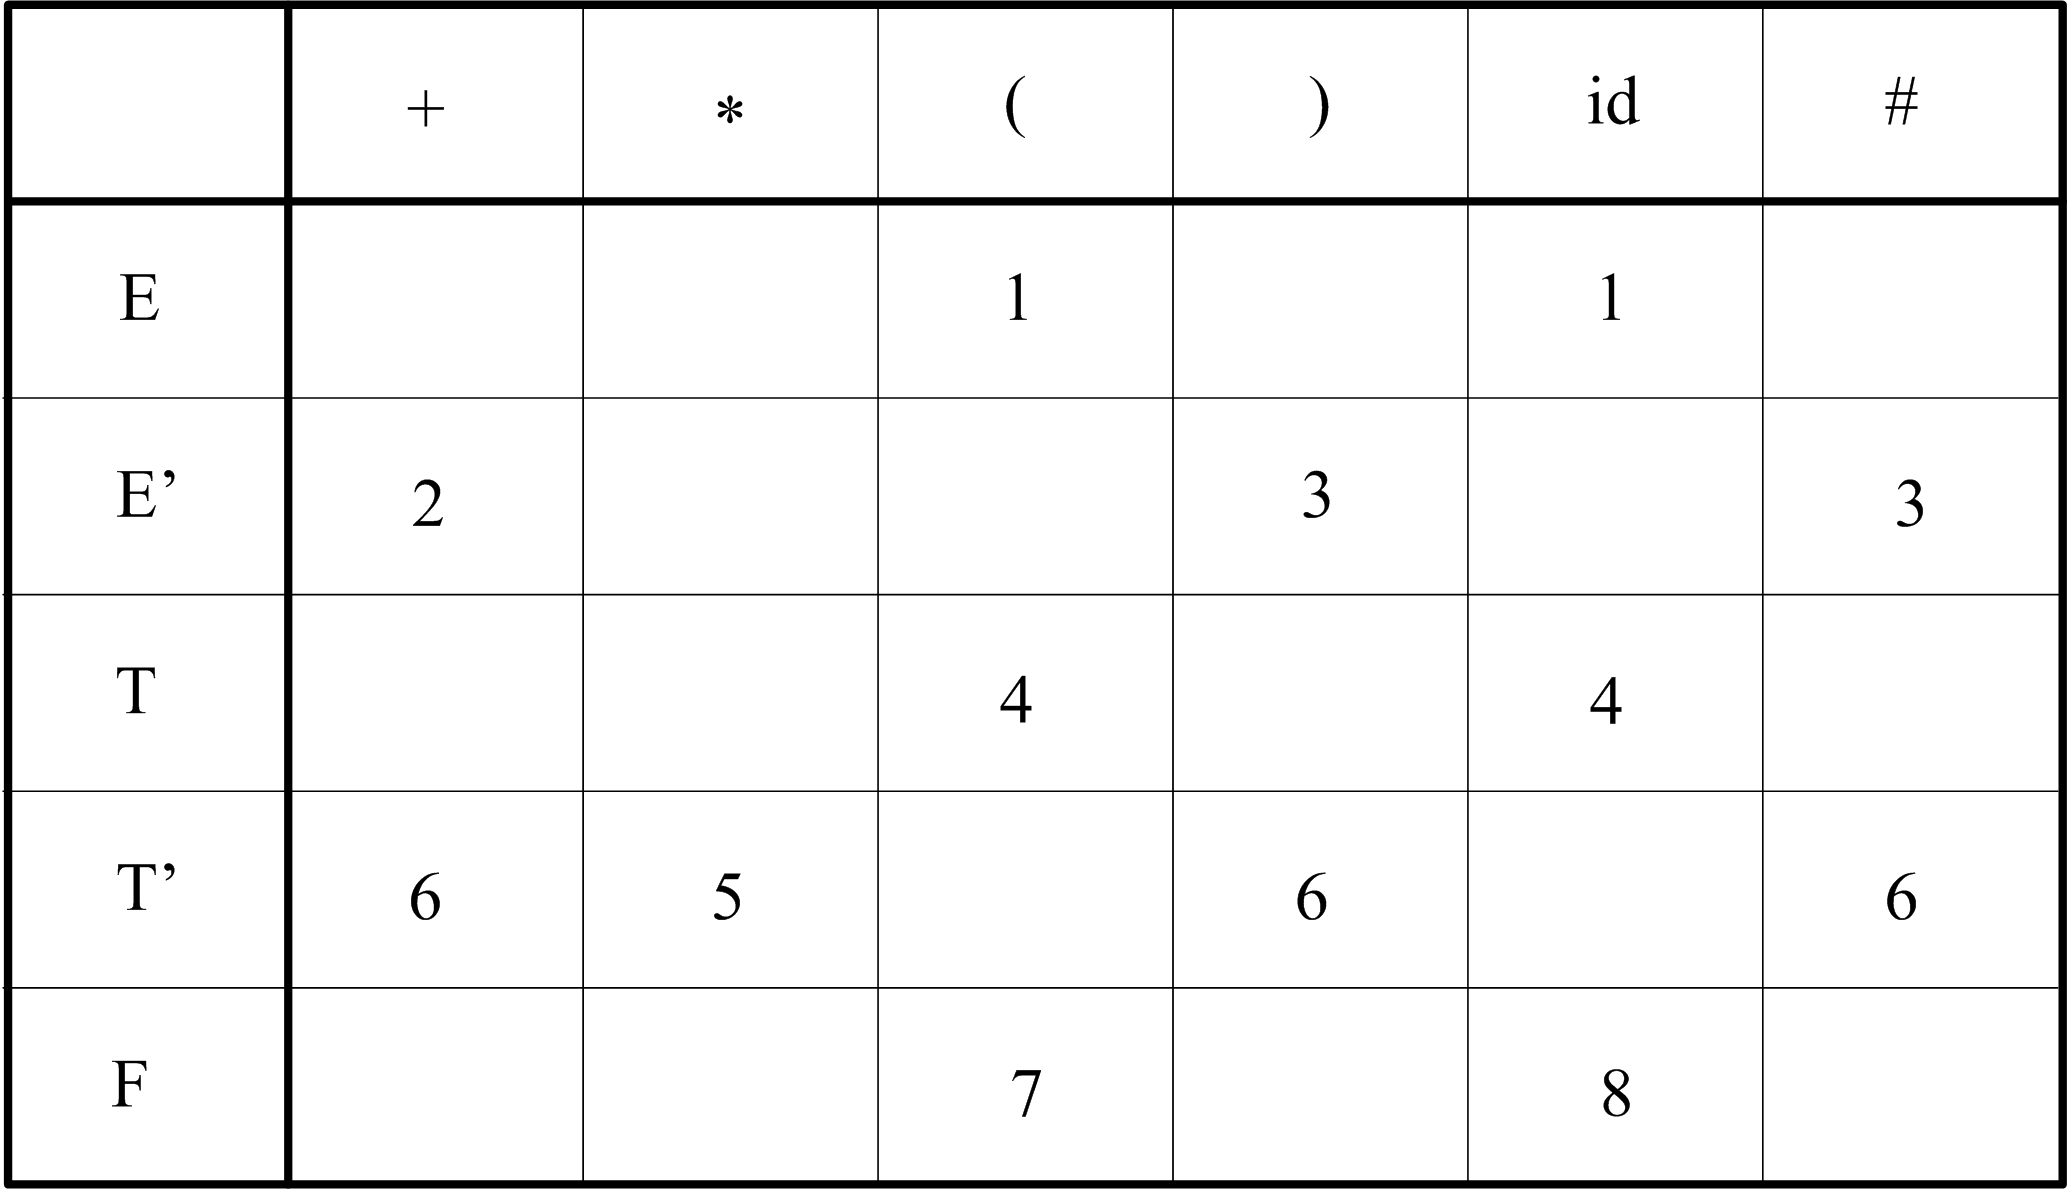
\includegraphics[scale=0.6]{{figures/figure03.05}.jpg}}
\end{center}

\pause
\bigskip

The LL(1) parsing algorithm is parameterized by this table, and makes use of an explicit pushdown stack

\pause

\begin{algorithm}[H]
\begin{algorithmic}
\REQUIRE LL(1) parse table $table$, production rules $rules$, and a sentence $w$, where $w$ is a string of terminals followed by a terminator \lstinline{#}
\ENSURE a left-parse, which is a left-most derivation for $w$
\end{algorithmic}
\caption{LL(1) Parsing Algorithm}
\end{algorithm}
\end{frame}

\begin{frame}[fragile]
\pause

\begin{algorithm}[H]
\begin{algorithmic}
\STATE Stack $stk$ initially contains the terminator \lstinline{#} and the start symbol $S$, with $S$ on top
\STATE Symbol $sym$ is the first symbol in the sentence $w$
\WHILE{true}
\STATE  Symbol $top \gets stk$.pop()
\IF{$top = sym =$ \lstinline{#}}
\STATE Halt successfully
\ELSIF{$top$ is a terminal symbol}
\IF{$top = sym$}
\STATE Advance $sym$ to be the next symbol in $w$
\ELSE
\STATE Halt with an error: a $sym$ found where a $top$ was expected
\ENDIF
\ELSIF{top is a non-terminal $Y$}
\STATE $index \gets table[Y, sym]$
\IF{$index \neq err$}
\STATE $rule \gets rules[index]$
\STATE Say rule is $Y ::= X_1X_2 \dots X_n$; push $X_n, \dots, X_2, X_1$ onto the stack $stk$, with $X_1$ on top
\ENDIF
\ELSE
\STATE Halt with an error
\ENDIF
\ENDWHILE
\end{algorithmic}
\caption{LL(1) Parsing Algorithm (contd.)}
\end{algorithm}
\end{frame}

\begin{frame}[fragile]
\pause

The steps in parsing \lstinline{id + id * id} against the above LL(1) parse table

\begin{center}
\visible<2->{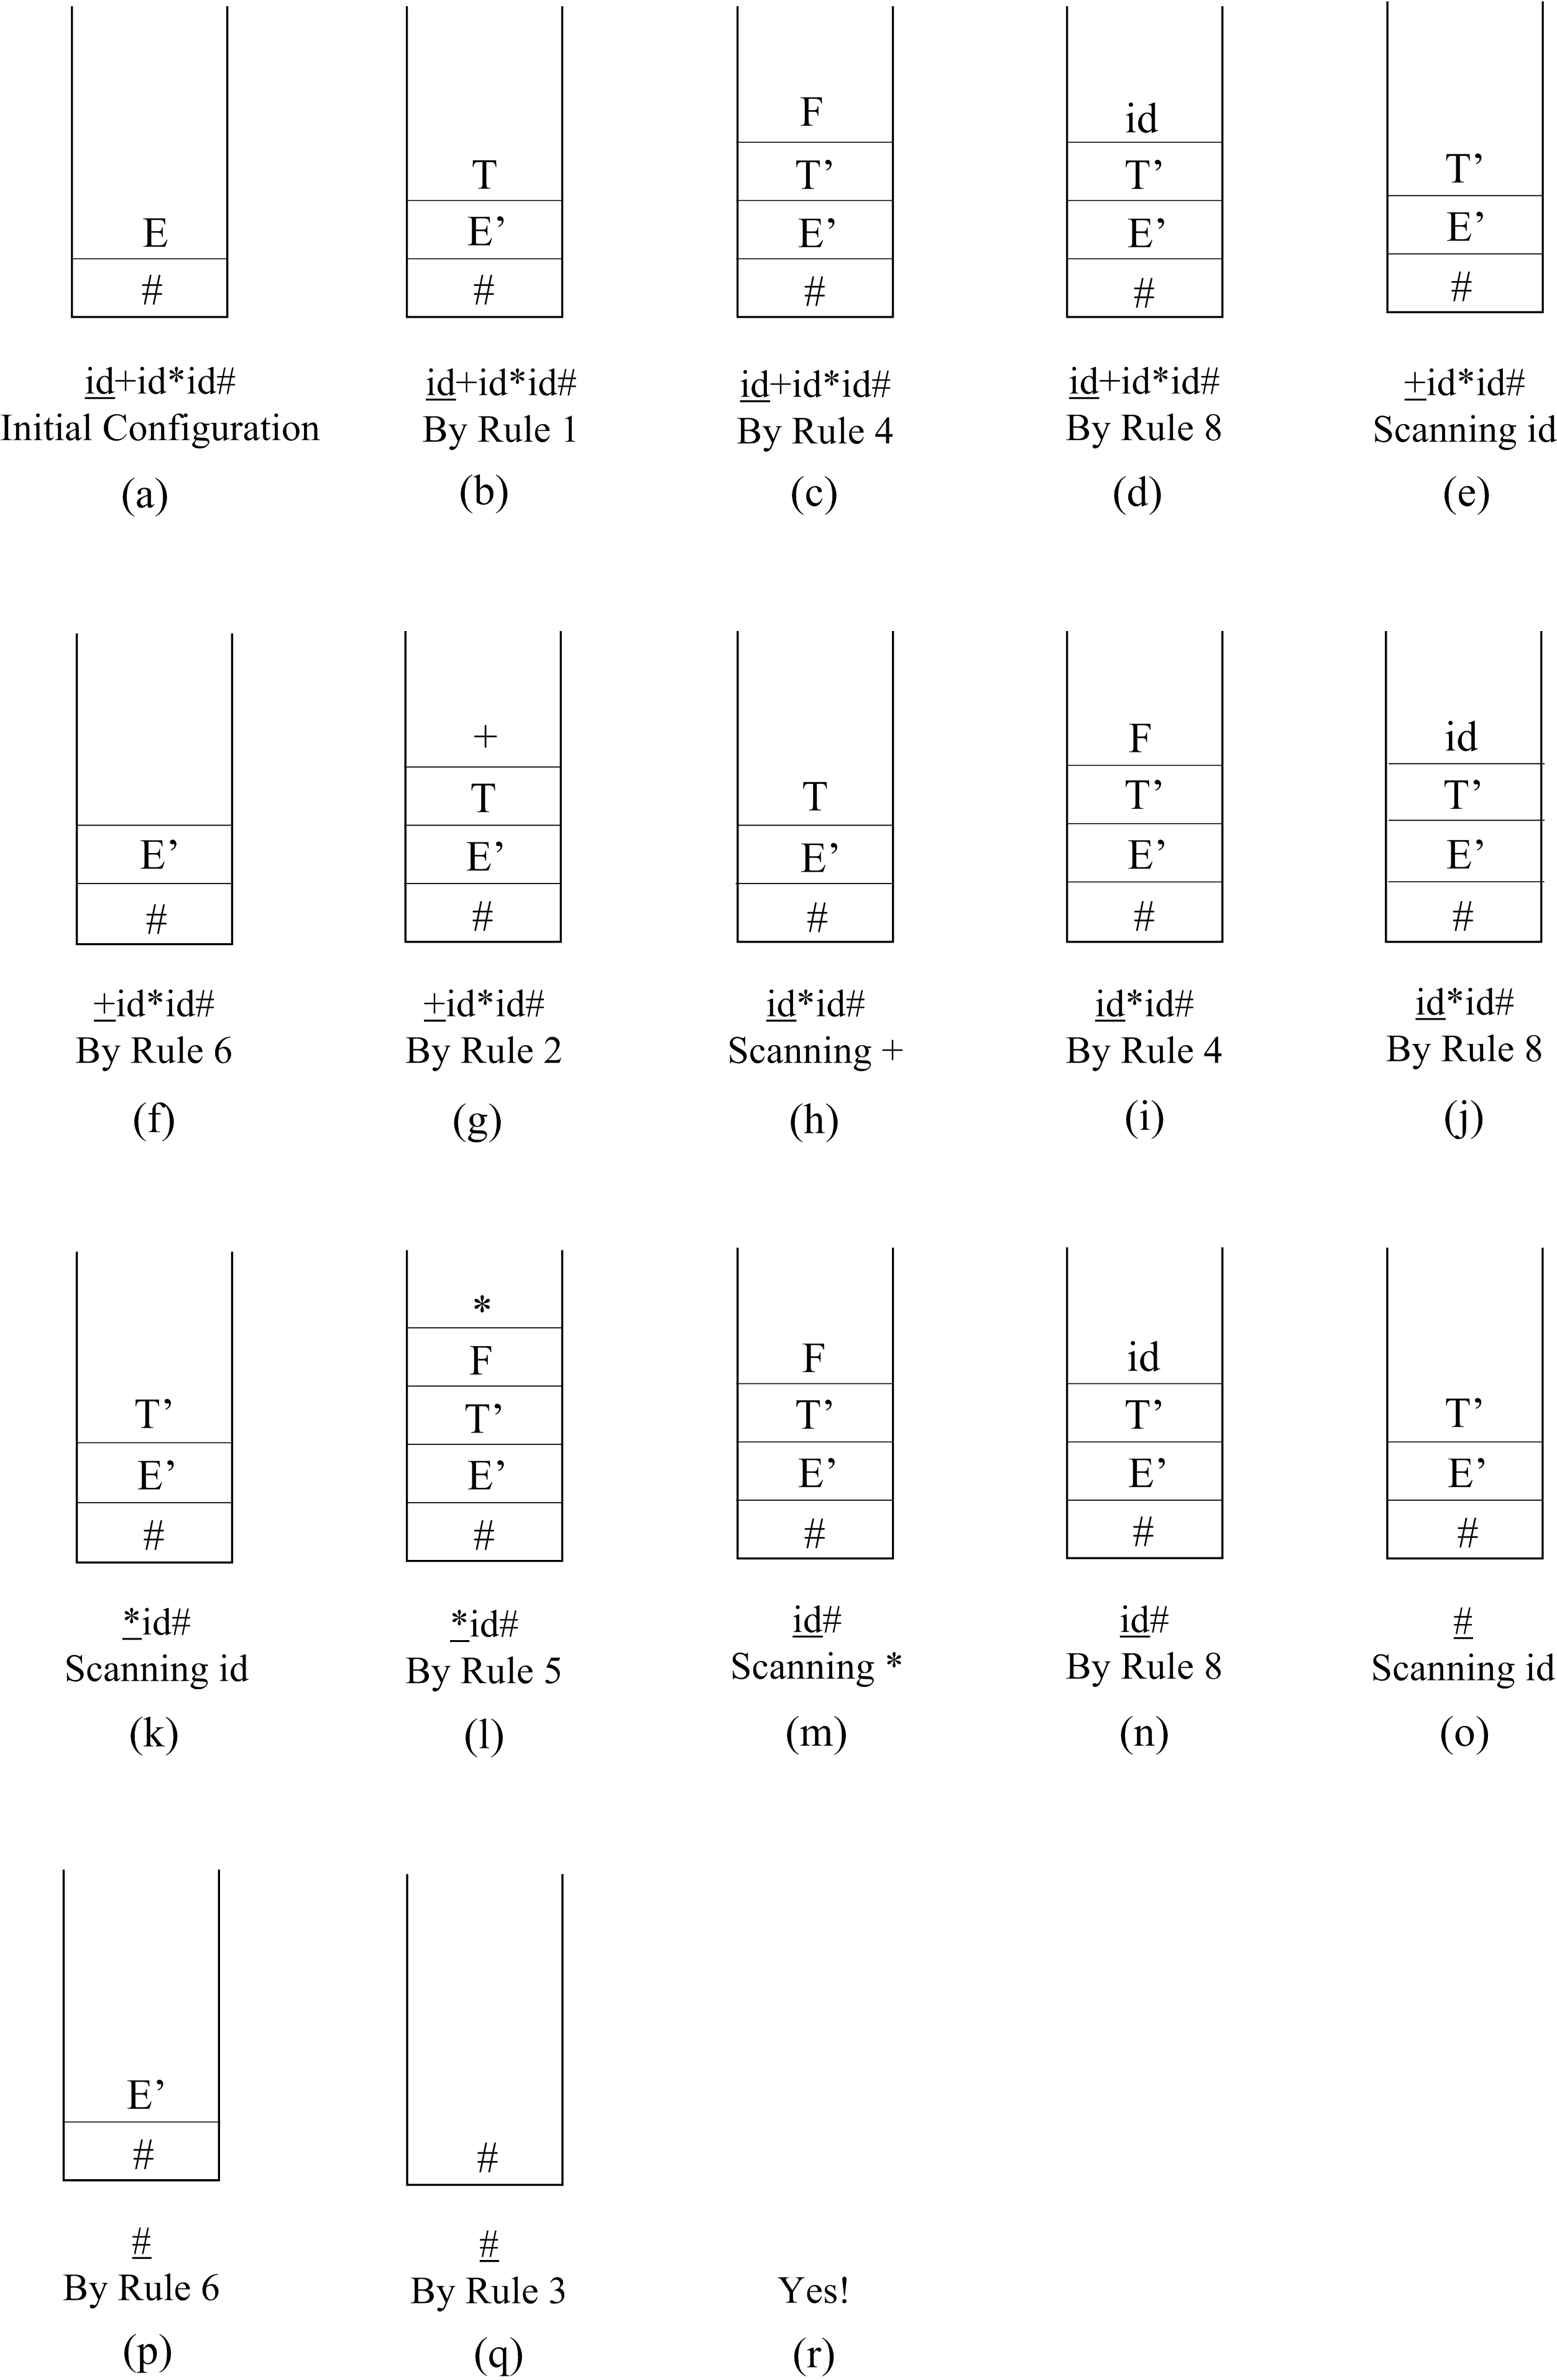
\includegraphics[scale=0.4]{{figures/figure03.06}.jpg}}
\end{center}
\end{frame}

\begin{frame}[fragile]
\pause

An alternative way of illustrating the states that the parser goes through is as follows

\begin{center}
\visible<2->{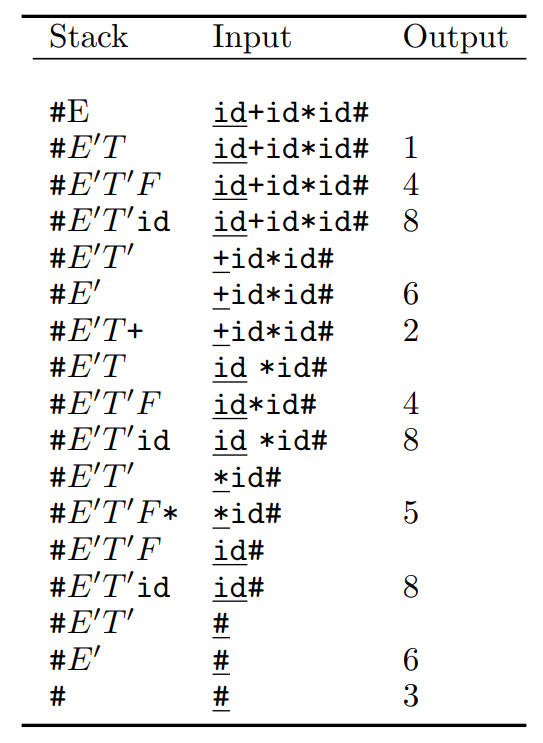
\includegraphics[scale=0.25]{{figures/figure03.06_alt}.jpg}}
\end{center}
\end{frame}

\begin{frame}[fragile]
\pause

How do we construct the LL(1) parse table?

\pause
\bigskip

\noindent table[$Y$, $a$] = $i$, where $i$ is the number of the rule $Y ::= X_1X_2 \dots X_n$

\bigskip

\noindent says that if there is the goal $Y$ on the stack and the next un-scanned symbol is $a$, then we can rewrite $Y$ on the stack as the sequence of sub goals $X_1X_2 \dots X_n$

\pause
\bigskip

When do we replace $Y$ with $X_1X_2 \dots X_n$ as opposed to something else?

\pause
\bigskip

If we consider the last two rules of our grammar

\text{ }
\begin{spaced}
\begin{production}
7. \mm{F} ::= \lstinline{(}\mm{E}\lstinline{)}
8. \mm{F} ::= \lstinline{id}
\end{production}
\end{spaced}

\noindent and we have the non-terminal $F$ on top of our parsing stack, the choice is simple; if the next un-scanned symbol is an open parenthesis \lstinline{(}, we apply rule 7, and if it is an \lstinline{id}, we apply rule 8, ie, 

\text{ }
\begin{spaced}
\begin{production}
table[\mm{F}, \lstinline{(}] = 7
table[\mm{F}, \lstinline{id}] = 8
\end{production}
\end{spaced}
\end{frame}

\begin{frame}[fragile]
\pause

The problem becomes slightly more complicated when the right-hand-side of the rule either starts with a non-terminal or is simply $\epsilon$

\pause
\bigskip

In general, assuming both $\alpha$ and $\beta$ are (possibly empty) strings of terminals and non-terminals, table[$Y$, $a$] = $i$, where $i$ is the number of the rule $Y ::= X_1X_2 \dots X_n$, if either

\begin{enumerate}
\item $X_1X_2\dots X_n \derives a\alpha$, or
\item $X_1X_2\dots X_n \derives \epsilon$, and there is a derivation S\lstinline{#} $\derives \alpha Y a\beta$, that is, $a$ can follow $Y$ in a derivation.
\end{enumerate}

\pause
\bigskip

For this we need two helper functions, first and follow

\pause
\bigskip

We define, $\text{first}(X_1X_2 \dots X_n) = \{a | X_1X_2 \dots X_n \derives a\alpha, a \in T\}$, ie, the set of all terminals that can start strings derivable from $X_1X_2 \dots X_n$; also, if $X_1X_2 \dots X_n \derives \epsilon$, then we say that $\text{first}(X_1X_2 \dots X_n)$ includes $\epsilon$

\pause
\bigskip

We define two algorithms for computing first: one for a single symbol and the other for a sequence of symbols; the two algorithms are both mutually recursive and make use of memoization, ie, what was previously computed for each set is remembered upon each iteration
\end{frame}

\begin{frame}[fragile]
\pause


\begin{algorithm}[H]
\begin{algorithmic}
\REQUIRE a context-free grammar $G = (N,T,S,P)$
\ENSURE first($X$) for all symbols $X$ in $G$
\FOR{each terminal $x$}
\STATE $\text{first}(x) \gets \{x\}$
\ENDFOR
\FOR{each non-terminal $X$}
\STATE $\text{first}(X) \gets \{\}$
\ENDFOR
\IF {$X ::= \epsilon \in P$}
\STATE add $\epsilon$ to $\text{first}(X)$
\ENDIF
\REPEAT
\FOR{each $Y ::= X_1X_2 \dots X_n \in P$}
\STATE add all symbols from $\text{first}(X_1X_2 \dots X_n)$ to $\text{first}(Y)$
\ENDFOR
\UNTIL{no new symbols are added to any set}
\end{algorithmic}
\caption{Compute first($X$) for all symbols $X$ in a Grammar $G$}
\end{algorithm}
\end{frame}

\begin{frame}[fragile]
\pause

\begin{algorithm}[H]
\begin{algorithmic}
\REQUIRE a context-free grammar $G = (N,T,S,P)$ and a sequence $X_1X_2 \dots X_n$
\ENSURE first($X_1X_2 \dots X_n$)
\STATE Set $S \gets \text{first}(X_1)$
\STATE $i \gets 2$
\WHILE{$\epsilon \in S$ and $i \le n$}
\STATE $S \gets S - \epsilon$
\STATE Add $\text{first}(X_i)$ to $S$
\STATE $i \gets i + 1$
\ENDWHILE
\RETURN $S$
\end{algorithmic}
\caption{Compute $\text{first}(X_1X_2 \dots X_n)$ for a Grammar $G$}
\end{algorithm}
\end{frame}

\begin{frame}[fragile]
\pause

Consider our example grammar

\text{ }
\begin{spaced}
\begin{production}
1. \mm{E}  ::= \mm{T} \expo{E}{\prime}
2. \expo{E}{\prime} ::= \lstinline{+} T \expo{E}{\prime}
3. \expo{E}{\prime} ::= \mm{\epsilon}
4. \mm{T}  ::= \mm{F} \expo{T}{\prime}
5. \expo{T}{\prime} ::= \lstinline{*} \mm{F} \expo{T}{\prime}
6. \expo{T}{\prime} ::= \mm{\epsilon}
7. \mm{F}  ::= \lstinline{(}\mm{E}\lstinline{)}
8. \mm{F}  ::= \lstinline{id}
\end{production}
\end{spaced}

\pause
\bigskip

The computation of first for the terminals, by step 1 of the first algorithm is trivial

\text{ }
\begin{spaced}
\begin{production}
first(\lstinline{+})  = \{\lstinline{\+}\}
first(\lstinline{*})  = \{\lstinline{*}\}
first(\lstinline{(})  = \{\lstinline{(}\}
first(\lstinline{)})  = \{\lstinline{)}\}
first(\lstinline{id}) = \{\lstinline{id}\}
\end{production}
\end{spaced}

\pause
\bigskip

Step 2 of the first algorithm gives

\text{ }
\begin{spaced}
\begin{production}
first(\mm{E})  = \{\}
first(\expo{E}{\prime}) = \{\}
first(\mm{T})  = \{\}
first(\expo{T}{\prime}) = \{\}
first(\mm{F})  = \{\}
\end{production}
\end{spaced}
\end{frame}

\begin{frame}[fragile]
\pause

Step 3 of the first algorithm yields

\text{ }
\begin{spaced}
\begin{production}
first(\expo{E}{\prime}) = \{\mm{\epsilon}\}
first(\expo{T}{\prime}) = \{\mm{\epsilon}\}
\end{production}
\end{spaced}

\pause

Step 4 of the first algorithm is repeatedly executed until no further symbols are added; the first round yields

\text{ }
\begin{spaced}
\begin{production}
first(E)  = \{\}
first(\expo{E}{\prime}) = \{\lstinline{+}, \mm{\epsilon}\}
first(\mm{T})  = \{\}
first(\expo{T}{\prime}) = \{\lstinline{*}, \mm{\epsilon}\}
first(\mm{F})  = \{\lstinline{\(}, \lstinline{id}\}
\end{production}
\end{spaced}

\pause

Second round of step 4 yields

\text{ }
\begin{spaced}
\begin{production}
first(\mm{E})  = \{\}
first(\expo{E}{\prime}) = \{\lstinline{\+}, \mm{\epsilon}\}
first(\mm{T})  = \{\lstinline{(}, \lstinline{id}\}
first(\expo{T}{\prime}) = \{\lstinline{\*}, \mm{\epsilon}\}
first(\mm{F})  = \{\lstinline{\(}, \lstinline{id}\}
\end{production}
\end{spaced}
\end{frame}

\begin{frame}[fragile]
\pause

Third round of step 4 yields

\text{ }
\begin{spaced}
\begin{production}
first(\mm{E})  = \{\lstinline{\(}, \lstinline{id}\}
first(\expo{E}{\prime}) = \{\lstinline{\+}, \mm{\epsilon}\}
first(\mm{T})  = \{\lstinline{(}, \lstinline{id}\}
first(\expo{T}{\prime}) = \{\lstinline{\*}, \mm{\epsilon}\}
first(\mm{F})  = \{\lstinline{\(}, \lstinline{id}\}
\end{production}
\end{spaced}

\pause

The fourth round of step 4 adds no symbols to any set, so we are done

\pause
\bigskip

When is a rule $X ::= \epsilon$ applicable?  For this we need the notion of follow

\pause
\bigskip

We define, $\text{follow}(X) = \{a | S \derives wX\alpha \text{ and } \alpha \derives a \dots\}$, ie, all terminal symbols that start terminal strings derivable from what can follow $X$ in a derivation

\pause
\bigskip

Another definition is as follows
\begin{enumerate}
\item $\text{follow}(S)$ contains \lstinline{#}, that is, the terminator follows the start symbol
\item If there is a rule $Y ::= \alpha X \beta$ in $P$, $\text{follow}(X)$ contains $\text{first}(\beta) - \{\epsilon\}$
\item If there is a rule $Y ::= \alpha X \beta$ in $P$ and either $\beta = \epsilon$ or $\text{first}(\beta)$ contains $\epsilon$, $\text{follow}(X)$ contains $\text{follow}(Y)$
\end{enumerate}
\end{frame}

\begin{frame}[fragile]
\pause

\begin{algorithm}[H]
\begin{algorithmic}
\REQUIRE a context-free grammar $G = (N,T,S,P)$
\ENSURE  $\text{follow}(X)$ for all non-terminals $X$ in $G$
\STATE $\text{follow}(S) \gets$ \{\lstinline{#}\}
\FOR{each non-terminal $X \in S$}
\STATE $\text{follow}(X) \gets \{\}$
\ENDFOR
\REPEAT
\FOR{each rule $Y ::= X_1X_2 \dots X_n \in P$}
\FOR{each non-terminal $X_i$}
\STATE Add $\text{first}(X_{i+1}X_{i+2} \dots X_n) - \{\epsilon\}$ to $\text{follow}(X_i)$, and
if $X_i$ is the right-most symbol or $\text{first}(X_{i+1}X_{i+2} \dots X_n)$ contains $\epsilon$, add $\text{follow}(Y)$ to $\text{follow}(X_i)$
\ENDFOR
\ENDFOR
\UNTIL{no new symbols are added to any set}
\end{algorithmic}
\caption{Compute $\text{follow}(X)$ for all non-terminals $X$ in a Grammar $G$}
\end{algorithm}
\end{frame}

\begin{frame}[fragile]
\pause

Again, consider our example grammar

\text{ }
\begin{spaced}
\begin{production}
1. \mm{E}  ::= \mm{T} \expo{E}{\prime}
2. \expo{E}{\prime} ::= \lstinline{+} T \expo{E}{\prime}
3. \expo{E}{\prime} ::= \mm{\epsilon}
4. \mm{T}  ::= \mm{F} \expo{T}{\prime}
5. \expo{T}{\prime} ::= \lstinline{*} \mm{F} \expo{T}{\prime}
6. \expo{T}{\prime} ::= \mm{\epsilon}
7. \mm{F}  ::= \lstinline{(}\mm{E}\lstinline{)}
8. \mm{F}  ::= \lstinline{id}
\end{production}
\end{spaced}

\pause

From rule 1, $E  ::= T E'$,  $\text{follow}(T)$ contains first($E'$) - $\{\epsilon\} = \{+\}$, and because first($E'$) contains $\epsilon$, it also contains follow($E$); also, follow($E'$) contains follow($E$); so, round 1 of step 3 yields,

\text{ }
\begin{spaced}
\begin{production}
follow(\expo{E}{\prime}) = \{\lstinline{#}\}
follow(\mm{T})  = \{\lstinline{+}, \lstinline{#}\}
\end{production}
\end{spaced}

\pause

We get nothing additional from rule 2, $E'$ ::= \lstinline{+} $T E'$; follow($T$) contains first($E'$) - $\{\epsilon\}$, but we saw that in rule 1; also, follow($E'$) contains follow($E'$), but that says nothing; we get nothing additional from rule 3, $E' ::= \epsilon$
\end{frame}

\begin{frame}[fragile]
\pause

From rule 4, $T  ::= F T'$, follow($F$) contains first($T'$) - $\{\}$ = \{\lstinline{*}\}, and because first($T'$) contains $\epsilon$, it also contains follow($T$); also, follow($T'$) contains follow($T$); so, we have

\text{ }
\begin{spaced}
\begin{production}
follow(\expo{T}{\prime}) = \{\lstinline{+}, \lstinline{#}\}
follow(\mm{F})  = \{\lstinline{+}, \lstinline{*}, \lstinline{#}\}
\end{production}
\end{spaced}

\pause

Rules 5 and 6 give us nothing new (for the same reasons rules 2 and 3 did not)

\pause
\bigskip

Rule 7, $F$  ::= \lstinline{(}$E$\lstinline{)}, adds \lstinline{)} to follow($E$), so

\text{ }
\begin{spaced}
\begin{production}
follow(\mm{E}) = \{\lstinline{)}, \lstinline{#}\}
\end{production}
\end{spaced}

\pause

Rule 8 gives us nothing

\pause
\bigskip

So round 1 of step 3 gives

\text{ }
\begin{spaced}
\begin{production}
follow(\mm{E})  = \{\lstinline{)}, \lstinline{#}\}
follow(\expo{E}{\prime}) = \{\lstinline{#}\}
follow(\mm{T})  = \{\lstinline{+}, \lstinline{#}\}
follow(\expo{T}{\prime}) = \{\lstinline{+}, \lstinline{#}\}
follow(\mm{F})  = \{\lstinline{+}, \lstinline{*}, \lstinline{#}\}
\end{production}
\end{spaced}
\end{frame}

\begin{frame}[fragile]
\pause

Now, in round 2 of step 3, the \lstinline{)} that was added to follow($E$) trickles down into the other follow sets

\pause
\bigskip

From rule 1, $E  ::= T E'$, because first($E'$) contains $\epsilon$, follow($T$) contains follow($E$); also, follow($E'$) contains follow($E$); so, we have

\text{ }
\begin{spaced}
\begin{production}
follow(\expo{E}{\prime}) = \{\lstinline{)}, \lstinline{#}\}
follow(\mm{T})  = \{\lstinline{+}, \lstinline{)},  \lstinline{#}\}
\end{production}
\end{spaced}

\pause

From rule 4, $T  ::= F T'$, because first($T'$) contains $\epsilon$, follow($F$) contains follow($T$); also, follow($T'$) contains follow($T$); so, we have

\text{ }
\begin{spaced}
\begin{production}
follow(\expo{T}{\prime}) = \{\lstinline{+}, \lstinline{)}, \lstinline{#}\}
follow(\mm{F})  = \{\lstinline{+}, \lstinline{*}, \lstinline{)}, \lstinline{#}\}
\end{production}
\end{spaced}

\pause

So round 2 produces

\text{ }
\begin{spaced}
\begin{production}
follow(\mm{E})  = \{\lstinline{)}, \lstinline{#}\}
follow(\expo{E}{\prime}) = \{\lstinline{)}, \lstinline{#}\}
follow(\mm{T})  = \{\lstinline{+}, \lstinline{)},  \lstinline{#}\}
follow(\expo{T}{\prime}) = \{\lstinline{+}, \lstinline{)}, \lstinline{#}\}
follow(\mm{F})  = \{\lstinline{+}, \lstinline{*}, \lstinline{)}, \lstinline{#}\}
\end{production}
\end{spaced}

\pause

Round 3 of step 3 adds no new symbols to any set, so we are done
\end{frame}

\begin{frame}[fragile]
\pause

Recall, assuming both $\alpha$ and $\beta$ are (possibly empty) strings of terminals and non-terminals, $\text{table}[Y, a] = i$, where $i$ is the number of the rule $Y ::= X_1X_2 \dots X_n$ if either

\begin{enumerate}
\item $X_1X_2 \dots X_n \derives a\alpha$, or
\item $X_1X_2 \dots X_n \derives \epsilon$, and there is a derivation $S$\lstinline{#} $\derives \alpha Ya\beta$, that is, $a$ can follow $Y$ in a derivation.
\end{enumerate}

This definition, together with the functions, first and follow, suggests the following algorithm for constructing the LL(1) parse table

\begin{algorithm}[H]
\begin{algorithmic}
\REQUIRE a context-free grammar $G=(N,T,S,P)$
\ENSURE LL(1) Parse Table for $G$
\FOR{each non-terminal $Y \in G$}
\FOR{each rule $Y ::= X_1X_2 \dots X_n \in P$ with number $i$}
\FOR{each terminal $a \in \text{first}(X_1X_2 \dots X_n) - \{\epsilon\}$}
\STATE $\text{table}[Y, a] \gets i$
\IF{$\text{first}(X_1X_2 \dots X_n)$ contains $\epsilon$}
\FOR{each terminal $a$ (or \lstinline{#}) in $\text{follow}(Y)$}
\STATE $\text{table}[Y, a] \gets i$
\ENDFOR
\ENDIF
\ENDFOR
\ENDFOR
\ENDFOR
\end{algorithmic}
\caption{Construct an LL(1) Parse Table for a Grammar $G=(N,T,S,P)$}
\end{algorithm}
\end{frame}

\begin{frame}[fragile]
\pause

Let us construct a parse table for our example grammar

\text{ }
\begin{spaced}
\begin{production}
1. \mm{E}  ::= \mm{T} \expo{E}{\prime}
2. \expo{E}{\prime} ::= \lstinline{+} T \expo{E}{\prime}
3. \expo{E}{\prime} ::= \mm{\epsilon}
4. \mm{T}  ::= \mm{F} \expo{T}{\prime}
5. \expo{T}{\prime} ::= \lstinline{*} \mm{F} \expo{T}{\prime}
6. \expo{T}{\prime} ::= \mm{\epsilon}
7. \mm{F}  ::= \lstinline{(}\mm{E}\lstinline{)}
8. \mm{F}  ::= \lstinline{id}
\end{production}
\end{spaced}

\pause

For the non-terminal $E$, we consider rule 1: $E  ::= T E'$.  first($T E'$) = \{\lstinline{(},\lstinline{id}\}; so, we have

\text{ }
\begin{spaced}
\begin{production}
table[\mm{E}, \lstinline{(}] = 1
table[\mm{E}, \lstinline{id}] = 1
\end{production}
\end{spaced}

\pause

Because first($T E'$) does not contain $\epsilon$, we need not consider follow($E$)

\pause
\bigskip

For the non-terminal $E'$, we first consider rule 2: $E'$ ::= \lstinline{+} $T E'$; first(\lstinline{+} $T$ $E'$) = \{\lstinline{+}\}, so we have

\text{ }
\begin{spaced}
\begin{production}
table[\expo{E}{\prime}, \lstinline{+}] = 2
\end{production}
\end{spaced}
\end{frame}

\begin{frame}[fragile]
\pause

Rule 3: $E' ::= \epsilon$ is applicable for symbols in follow($E'$) =  \{\lstinline{)}, \lstinline{#}\}, so we have

\text{ }
\begin{spaced}
\begin{production}
table[\expo{E}{\prime}, \lstinline{)}] = 3
table[\expo{E}{\prime}, \lstinline{#}] = 3
\end{production}
\end{spaced}

\pause

For the non-terminal $T$, we consider rule 4: $T  ::= F T'$. first($F$ $T'$) = \{\lstinline{(}, \lstinline{id}\}, so we have

\text{ }
\begin{spaced}
\begin{production}
table[\mm{T}, \lstinline{(}] = 4
table[\mm{T}, \lstinline{id}] = 4
\end{production}
\end{spaced}

\pause

Because first($F$ $T'$) does not contain $\epsilon$, we need not consider follow($T$)

\pause
\bigskip

For non-terminal $T'$, we first consider rule: 5: $T'$ ::= \lstinline{*} $F T'$; first(\lstinline{*} $F$ $T'$), so we have

\text{ }
\begin{spaced}
\begin{production}
table[\expo{T}{\prime}, \lstinline{*}] = 5
\end{production}
\end{spaced}

\pause

Rule 6: $T' ::= \epsilon$ is applicable for symbols in follow($T'$) = \{\lstinline{+}, \lstinline{)}, \lstinline{#}\}, so we have

\text{ }
\begin{spaced}
\begin{production}
table[\expo{T}{\prime}, \lstinline{+}] = 6
table[\expo{T}{\prime}, \lstinline{)}] = 6
table[\expo{T}{\prime}, \lstinline{#}] = 6
\end{production}
\end{spaced}
\end{frame}

\begin{frame}[fragile]
\pause

For the non-terminal $F$, we have two rules: Firstly, given rule 7: $F$  ::= \lstinline{(}$E$\lstinline{)}, and that first(\lstinline{(}$E$\lstinline{)}) = \{\lstinline{(}\},

\text{ }
\begin{spaced}
\begin{production}
table[\mm{F}, \lstinline{(}] = 7
\end{production}
\end{spaced}

\pause

Secondly, given rule 8: $F$  ::= \lstinline{id}, and since (obviously) first(\lstinline{id}) = \{\lstinline{id}\},

\text{ }
\begin{spaced}
\begin{production}
table[\mm{F}, \lstinline{id}] = 8
\end{production}
\end{spaced}

\pause

We say a grammar is LL(1) if the parse table has no conflicts, ie, no entries having more than one rule

\pause
\bigskip

If a grammar is shown to be LL(1) then it is unambiguous

\pause
\bigskip

It is possible for a grammar not to be LL(1) but LL($k$) for some $k > 1$; in principle, this would mean a table having columns for each combination of $k$ symbols

\pause
\bigskip

On the other hand, an LL(1) parser generator (JavaCC for example) based on the table construction algorithm, might allow one to specify a $k$-symbol look ahead for specific non-terminals or rules; these special cases can be handled specially by the parser and so need not lead to overly large (and, most likely sparse) tables
\end{frame}

\begin{frame}[fragile]
\pause

Not all context-free grammars are LL(1), but for many that are not, one may define equivalent grammars that are LL(1)

\pause
\bigskip

One class of grammar that is not LL(1) is a grammar having a rule with left recursion; for example 

\text{ }
\begin{spaced}
\begin{production}
Y ::= Y \mm{\alpha}
Y ::= \mm{\beta}
\end{production}
\end{spaced}

\pause

Clearly, a grammar having these two rules is not LL(1), because, by definition, first($Y \alpha$) must include first($\beta$) making it impossible to discern which rule to apply for expanding $Y$

\pause
\bigskip

Introducing an extra non-terminal, an extra rule, and replacing the left recursion with right recursion easily removes the direct left recursion

\text{ }
\begin{spaced}
\begin{production}
Y  ::= \mm{\beta} \expo{Y}{\prime}
\expo{Y}{\prime} ::= \mm{\alpha} \expo{Y}{\prime}
\expo{Y}{\prime} ::= \mm{\epsilon}
\end{production}
\end{spaced}
\end{frame}

\begin{frame}[fragile]
\pause

For example, consider the following context-free grammar

\text{ }
\begin{spaced}
\begin{production}
\mm{E} ::= \mm{E} \lstinline{+} \mm{T}
\mm{E} ::= \mm{T}
\mm{T} ::= \mm{T}  \lstinline{*} {F}
\mm{T} ::= \mm{F}
\mm{F} ::= \lstinline{(}\mm{E}\lstinline{)}
\mm{F} ::= \lstinline{id}
\end{production}
\end{spaced}

\pause

The left recursion captures the left-associative nature of the operators \lstinline{+} and \lstinline{*}, but because the grammar has left-recursive rules, it is not LL(1); we may apply the left-recursion removal rule to this grammar

\pause
\bigskip

Firstly, applying the rule to $E$ to produce

\text{ }
\begin{spaced}
\begin{production}
\mm{E}  ::= \mm{T} \expo{E}{\prime}
\expo{E}{\prime} ::= \lstinline{+} \mm{T} \expo{E}{\prime}
\expo{E}{\prime} ::= \mm{\epsilon}
\end{production}
\end{spaced}
\end{frame}

\begin{frame}[fragile]
\pause

Applying the rule to $T$ yields

\text{ }
\begin{spaced}
\begin{production}
\mm{T}  ::= \mm{F} \expo{T}{\prime}
\expo{T}{\prime} ::= \lstinline{*} \mm{F} \expo{T}{\prime}
\expo{T}{\prime} ::= \mm{\epsilon}
\end{production}
\end{spaced}

\pause

Giving us the LL(1) grammar

\text{ }
\begin{spaced}
\begin{production}
\mm{E}  ::= \mm{T} \expo{E}{\prime}
\expo{E}{\prime} ::= \lstinline{+} \mm{T} \expo{E}{\prime}
\expo{E}{\prime} ::= \mm{\epsilon}
\mm{T}  ::= \mm{F} \expo{T}{\prime}
\expo{T}{\prime} ::= \lstinline{*} \mm{F} \expo{T}{\prime}
\expo{T}{\prime} ::= \mm{\epsilon}
\mm{F}  ::= \lstinline{(}\mm{E}\lstinline{)}
\mm{F}  ::= \lstinline{id}
\end{production}
\end{spaced}
\end{frame}

\begin{frame}[fragile]
\pause

\begin{algorithm}[H]
\begin{algorithmic}
\REQUIRE a context-free grammar $G=(N,T,S,P)$
\ENSURE $G$ with left recursion eliminated
\STATE Arbitrarily enumerate the non-terminals of $G: X_1, X_2, \dots, X_n$
\FOR{$i := 1 \text{ to } n$}
\FOR{$j := 1 \text{ to } i - 1$}
\STATE Replace each rule in $P$ of the form $X_i::= X_j\alpha$ by the rules $X_i ::= \beta_1\alpha | \beta_2\alpha | \dots | \beta_k\alpha$ where $X_j ::= \beta_1 | \beta_2 | \dots | \beta_k$ are the current rules defining $X_i$
\STATE Eliminate any immediate left recursion using (3.25)
\ENDFOR
\ENDFOR
\end{algorithmic}
\caption{Left Recursion Removal for a Grammar $G=(N,T,S,P)$}
\end{algorithm}
\end{frame}

\begin{frame}[fragile]
\pause

\end{frame}

\section{Bottom-up Deterministic Parsing}
\begin{frame}[fragile]
\pause

\end{frame}

\section{Parser Generation Using JavaCC}
\begin{frame}[fragile]
\pause

\end{frame}
\end{document}
